\clearpage
\section{The solution space and exit-time limits}\label{chap:solutions}

This chapter has three main goals. Firstly, following the well-posedness analysis of \autoref{chap:wellposed}, \autoref{thm:include_zero} provides a condition applicable to \autoref{prob:ivp} which preserves results thus far and also accommodates initial values where $\vp'(\tau)=f(\tau,\xi) = 0$, rather than $f(\tau,\xi)>0$. Despite having negligible modelling consequences, \autoref{thm:include_zero} both instils harmony in our IVPs' solution space, and provides a tangible interpretation on why the maximal uniqueness result of \autoref{thm:global_uniqueness} holds despite $f(t,\vp(t)) = 0$ being possible for any future time $t>\tau$.

As with \autoref{chap:wellposed}, the subdomain $[\tau,\infty)\times[\xi,\infty)\subset\RR^2$ of a function $f\in\uF\subset\uC(\RR^2,\RR)$ determines the behaviour of solutions, so to avoid repetition of assumptions, the pragmatic conclusion of \autoref{sec:refining_problem} is to simplify the IVPs being considered, to be driven by related functions $g\in\uG\subset\uC(\RR_+^2,\RR)$ like the Heston example in \autoref{eq:hest_ode}. Having treated initial values with due care, only IVPs of type $x'=g(t,x)$, $x(0)=0$ are then w.l.o.g.~considered.

Such IVPs feature in \autoref{prob:ivp2}, and with this the modelling foundations for the remainder of the thesis are set. The second goal of this chapter is to precisely understand the solution set of these IVPs, and how certain discontinuous limit points can arise through simple sequences of them. This analysis takes us to \autoref{sec:bounds_limits} which, via \autoref{thm:exit_limit}, provides foundations for understanding surprising limiting relationship between the time-integrated CIR process and L\'evy subordinators such as the IG process from \autoref{eq:ig_intro}. But more generally a simple recipe is provided to construct \emph{any} strictly increasing and unbounded path in $\uD(\RR_+,\RR_+)$ as a limit of IVP solutions on an intuitive `exit-time' metric space $(\bPhi,d_{\bPhi})$.

The final goal of this chapter is to expose the consequences of such limits $\vp_n\xrightarrow{n\to\infty}\vp_0$ on $(\bPhi,d_{\bPhi})$ for composite paths $w\circ\vp_n$, for any $w\in\uC(\RR_+,\RR)$. The composite convergence $w\circ\vp_n\xrightarrow{n\to\infty}w\circ\vp_0$ takes place pointwise a.e., but is violated on Skorokhod's topologies because $w\circ\vp_n$ can develop instantaneous `excursions' as $n\to\infty$. So in \autoref{sec:excursionary_limits} a Hausdorff metric space $(\uE,d_\uE)$ is introduced on which convergence of graphs is established. This provides the foundations to answer questions in the \hyperlink{prologue}{Prologue} on the Heston and NIG relationship, eventually extending \autoref{thm:mech_pro} to a practically valuable functional result.

With this pathwise theory in place, we will be ready to move to the probabilistic framework of \autoref{chap:framework} in which the results thus far, relating to IVP solutions $\vp$, will apply a.s.~to cumulative variance and price processes, $X$ and $S$. As outlined in \autoref{ch:intro}, these will be related through a \emph{composition} $S=\exp(W^\rho_X-\frac12 X)$, hence our emphasis on composite paths.

\subsection{Simplifying the problem}\label{sec:refining_problem}

In \autoref{chap:wellposed}, only IVPs $x'=f(t,x)$, $x(\tau)=\xi$ with initial values $(\tau,\xi)\in\RR^2$ where $f(\tau,\xi)>0$ were considered, meaning that a solution $\vp$ verifies $\vp'(\tau)=f(\tau,\xi)>0$. However, the maximal uniqueness result of \autoref{thm:global_uniqueness} accommodates times $t>\tau$ where $\vp'(t)=f(t,\vp(t))=0$, suggesting some naturally occurring conditions where $f(\tau_*,\xi_*)=0$ for some $\tau_*>\tau$ and $\xi_*>\xi$, yet uniqueness of the translated IVP $x'=f(t,x)$, $x(\tau_*)=\xi_*$ still holds.

Indeed, a consequence of \autoref{thm:include_zero} here is that:~provided the point $(\tau,\xi)\in\RR^2$ is attainable by some strictly increasing (`history') $\vp\in\uC^1((T,\tau],\RR)$ which solves the \emph{terminal} value problem $x'=f(t,x)$, $x(\tau)=\xi$, then there exists a unique maximal solution (`future') of the corresponding \emph{initial} value problem, whether $f(\tau,\xi)=0$ or not. This natural stability is peculiar, given the forthcoming counterexamples to uniqueness when $f(\tau,\xi)=0$ in general.

Following these counterexamples and the proof of \autoref{thm:include_zero}, the new set of IVP functions $\uG\subset\uC(\RR_+^2,\RR)$ introduced in \autoref{ch:intro} is properly defined, which will be prioritised in the remainder of this chapter and taken into \autoref{chap:framework}. Although this set $\uG$ is not quite as simple to define as $\uF$, the related maximal solutions $\vp$ are certainly simpler to analyse. This is primarily because these always constitute differentiable bijections from and to $\RR_+$, so maximal solutions are in fact global. As discussed, this is very helpful when moving to a probabilistic setting, given requirements to understand the solution space topologically.

\vspace{3mm}\textbf{Non-uniqueness examples.} Recall the common counterexample to IVP uniqueness given by $x'=f(t,x):=|x|^\alpha$, $x(0)=0$ for some $\alpha\in(0,1)$. It is straightforward to verify the two global solutions $\vp_\infty(t):=0$ and $\vp_0(t):=((1-\alpha)t)^\frac{1}{1-\alpha}$, and to combine these to get others,
\begin{equation}\label{eq:standard_nonunique}
    \vp_T(t) :=
    \begin{cases}
        \vp_\infty(t) & t\in[0,T),\\
        \vp_0(t-T) & t\in[T,\infty),
    \end{cases}
\end{equation}
for any $T\in(0,\infty)$. Indeed, the convergences $\vp_T\xrightarrow{T\downarrow 0}\vp_0$ and  $\vp_T\xrightarrow{T\uparrow\infty}\vp_\infty$ then take place uniformly over compacts. The point of raising this example is to clarify that, in our case where $f\in\uF$, we do not need to worry about this translation of solutions along a line like $x=0$ here. This is because such lines, where $f(\cdot,x)$ is necessarily zero, are precluded by the condition that every $f(\cdot,x)$ is strictly increasing. However, notice that when this IVP is adapted to $x'=\sgn(x)|x|^\alpha$, $x(0)=0$, then we get additional \emph{negative} solutions like $-\vp_0$. These are precisely the kind of non-uniqueness examples which we \emph{do} need to worry about.

For a thorough extension of these cases to our setting, we could consider functions of type
\begin{equation}
    f(t,x) := I_{a,b}(t)|t|^\alpha + I_{c,d}(x)|x|^\beta,\quad I_{a,b}(t):=a\mathbbm{1}_{t<0} + b\mathbbm{1}_{t\ge0}
\end{equation}
for $a,b,c,d\in\RR$ and $\alpha,\beta\in(0,1)$. Notice that $f\in\uF$ provided that $a<0<b$, given every $f(\cdot,x)$ is then strictly increasing. Checking that $I_{c,d}(x)=\sgn(x)$ when $(c,d)=(-1,1)$, it is interesting to note that we can still get non-uniqueness without this ordering $c<0<d$.

For the sake of clarity, we will just consider cases $f\in\uF$ with the simplified representation
\begin{equation}\label{eq:nonunique_example}
    f(t,x) := t + I_{a,b}(x)\sqrt{|x|}
\end{equation}
for some $a,b\in\RR$. Notice that the IVP $x'=f(t,x)$, $x(\tau)=0$ then provides an example of \autoref{prob:ivp} whenever $\tau>0$ because $f(\tau,0)=\tau>0$, contrasting $\tau=0$ given $f(0,0)=0$.

In the case of $-3=:a<0<b:=1$ and $\tau=0$, we get the two parabolic solutions $\vp_{\pm}(t):=\pm t^2$, which is straightforward to confirm. But even if we set $-3=:a<b:=-1<0$, so the sign of $I_{a,b}$ no longer changes over the line $x=0$, we still get two solutions, namely $\vp_+(t)=\frac14 t^2$ and $\vp_-(t)=-t^2$. The solutions $\vp_\pm$ for these examples are demonstrated in \autoref{fig:nonuniqueness}, also with the path $\phi(x):=-I_{a,b}(x)\sqrt{|x|}$ from \autoref{lem:zeros1}, where $f(\phi(x),x)=0$.

\begin{figure}[ht]
    \centering
    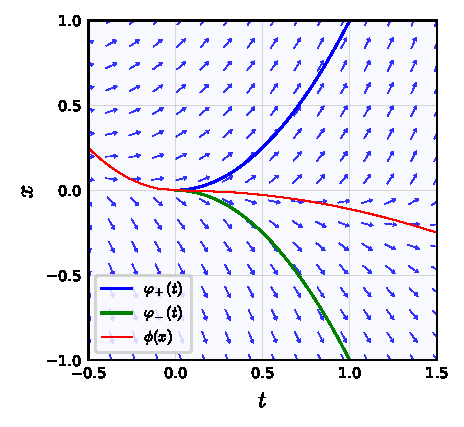
\includegraphics[width=0.48\linewidth]{figures/nonuniqueness1}
    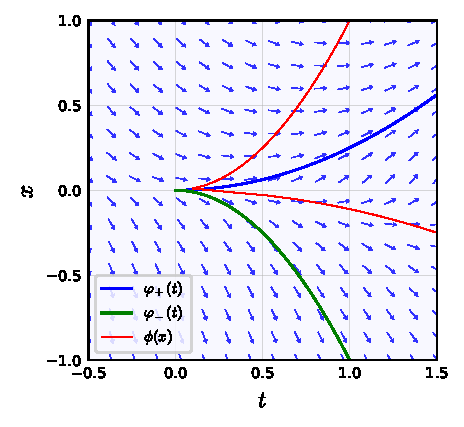
\includegraphics[width=0.48\linewidth]{figures/nonuniqueness2}
    \caption{The functions $f(t,x)$ (blue arrows) from \autoref{eq:nonunique_example}, where $(a,b)=(-3,1)$ in the left panel and $(a,b)=(-3,-1)$ in the right panel. The two solutions $\vp_\pm(t)$ of the IVP $x'=f(t,x)$, $x(0)=0$ are shown, with the path $\phi(x) = - I_{a,b}(x)\sqrt{|x|}$.}
    \label{fig:nonuniqueness}
\end{figure}

So while the results of \autoref{chap:wellposed} apply to these examples from \autoref{eq:nonunique_example} when $\tau>0$, few do when $\tau=0$. This clearly demonstrates that we cannot in general relax the condition $f(\tau,\xi)>0$ in the statement of \autoref{prob:ivp} to $f(\tau,\xi)\ge0$, and retain well-posedness qualities.

Following this breakdown of uniqueness, it is straightforward to construct examples of `discontinuous dependence', violating \autoref{thm:continuity_solution_map}. For example, let the function $f_0$ be defined as in \autoref{eq:nonunique_example} with $(a,b)=(-3,1)$ and take the global solution $\vp_0(t):=-t^2$ of the IVP $x'=f_0(t,x)$, $x(0)=0$. Then define $f_n(t,x):=f_0(t+n^{-1},x)$ which generates unique global parabolic solutions $\vp_n(t):=(t+\frac12 n^{-1})^2$. Now clearly $\Vert f_0-f_n \Vert_{[0,T]\times[0,X]}\xrightarrow{n\to\infty}0$ for all $T,X>0$, as per the conditions of \autoref{thm:continuity_solution_map}, but we find $\Vert\vp_0-\vp_n\Vert_{[0,T]}\xrightarrow{n\to\infty}2T^2$. This distance $2T^2$ is nothing but the difference $\vp_+(T)-\vp_-(T)$ in the left panel of \autoref{fig:nonuniqueness}.

Before proceeding, it is worth making two pragmatic remarks. Firstly, it is practically reassuring that the forward Euler scheme of \autoref{alg:forward_euler} will not only converge for any example like these, but will converge to the desirable strictly increasing solution. This is to say, \autoref{thm:euler_converge} still holds when $f(\tau,\xi)=0$. This is straightforward to see with \autoref{fig:nonuniqueness} in mind; if $f(\tau,\xi)=0$, then any $\pi$-polygon for the IVP $x'=f(t,x)$, $x(\tau)=\xi$ satisfies $\vp_\pi(t_1)=\vp_\pi(t_0) + (t_1-t_0)\times 0=\xi$, and then $\vp_\pi(t_2)=\vp_\pi(t_1) + (t_1-t_0)f(t_1,\vp_\pi(t_1)) = \xi + (t_1-\tau)f(t_1,\xi)>\xi$, given $t_1>\tau$ and $f(\cdot,\xi)$ is strictly increasing. Such polygons thus converge to the \emph{strictly increasing} limit as $\Vert\pi\Vert\to0$, for the same reasons as in \autoref{thm:euler_converge}.

Secondly, it is worth at this point noticing in
\autoref{fig:nonuniqueness} that, given one finds $f(t,x)<0$ in all of $(-\infty,\tau)\times(-\infty,\xi)$, there can clearly be no strictly increasing solution $\vp\in\uC^1((T,\tau],\RR)$ to the TVP $x'=f(t,x)$, $x(\tau)=\xi$ when $(\tau,\xi)=(0,0)$, i.e.~no physically meaningful `history' which arrives at the point $(0,0)$. This renders $(0,0)$ an unnatural initial value to choose, given we cannot make sense of volatility $\sqrt{\vp'}$ in the past. We only have to reverse the sign of $a$ in \autoref{fig:nonuniqueness} to avoid this, as \autoref{fig:nonuniqueness2} illustrates. But the right hand panel of \autoref{fig:nonuniqueness2} shows that, as a result, uniqueness can now be violated going \emph{backwards} in time from $(0,0)$, which justifies earlier remarks related to the time-irreversibility of the IVPs considered here.

\begin{figure}[ht]
    \centering
    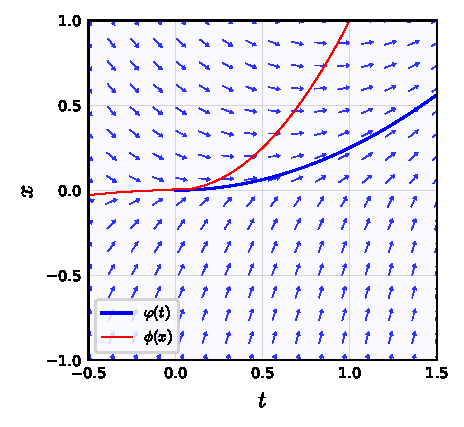
\includegraphics[width=0.48\linewidth]{figures/nonuniqueness3}
    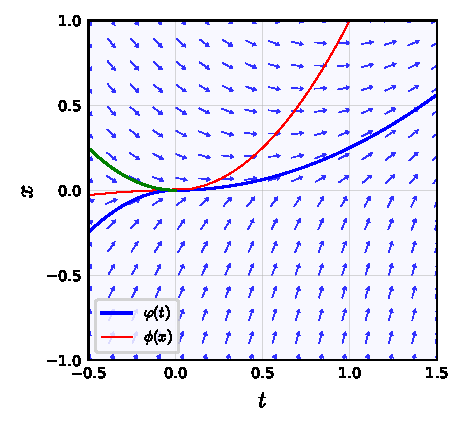
\includegraphics[width=0.48\linewidth]{figures/nonuniqueness4}
    \caption{A repeat of the right panel of \autoref{fig:nonuniqueness}, with instead $(a,b)=(3,-1)$. Now a physically meaningful (strictly increasing) TVP solution which arrives at $(0,0)$ exists over $-\RR_+$, and the corresponding IVP has a unique global solution over $\RR_+$.}
    \label{fig:nonuniqueness2}
\end{figure}

\vspace{3mm}\textbf{Conditions enabling $\boldsymbol{f(\tau,\xi)=0}$.} We now provide a condition which ensure we are in the setting of \autoref{fig:nonuniqueness2} rather than \autoref{fig:nonuniqueness} when selecting initial values $(\tau,\xi)$. While there may not be a unique solution arriving at $(\tau,\xi)$ from the past, this will ensure there is always a unique and physically meaningful solution into the future. It is important to recognise that this condition is applicable to the general setting of \autoref{chap:wellposed} where $f\in\uF$, and not just the visually helpful examples just covered. The relatively simple functions $I_{a,b}(x)\sqrt{x}$ from \autoref{eq:nonunique_example} could therefore be replaced by any path $w\in\uC(\RR,\RR)$, like those from \autoref{ex:main_example}, and these problematic points, like $x=0$ in \autoref{fig:nonuniqueness}, could be dense in $\RR$.

The forthcoming condition of \autoref{thm:include_zero} applies to the triple $(f,\tau,\xi)\in\uF\times\RR^2$ and is geometrically intuitive, given \autoref{fig:nonuniqueness2}. Following this, a more abstract interpretation of this condition, in terms of the path $\phi\in\uC(\RR,\bRR)$ of zeros from \autoref{lem:zeros1}, is given. First, for each initial value $(\tau,\xi)\in\RR^2$ and $c\in\RR$, $\ep>0$, let the line $\cX_{c,\ep}(\tau,\xi)\subset\RR^2$ be defined by
\begin{equation}\label{eq:line_def}
    \cX_{c,\ep}(\tau,\xi) := \{(\tau+cx,\xi-x):x\in(0,\ep)\}.
\end{equation}

\begin{theorem}[Additional initial values]\label{thm:include_zero}
    All of the results of \autoref{chap:wellposed}, relating to an IVP $x'=f(t,x)$, $x(\tau)=\xi$ with $f\in\uF$ and $f(\tau,\xi)>0$, hold if the requirement `$f(\tau,\xi)>0$' is replaced by the existence of any line $\cX_{c,\ep}(\tau,\xi)$ such that $f(t,x)>0$ for all $(t,x)\in\cX_{c,\ep}(\tau,\xi)$.
\end{theorem}
\begin{proof}
    There is nothing to prove if $f(\tau,\xi)>0$. The assumption that $f(t,x)>0$ on some such line $\cX_{c,\ep}(\tau,\xi)$ precludes $f(\tau,\xi)<0$ by the continuity of $f$, so now suppose $f(\tau,\xi)=0$.

    In \autoref{chap:wellposed} we swiftly concluded that any maximal solution $\vp\in\uC^1([\tau,T_*),\RR)$ is strictly increasing, in \autoref{thm:bijectivity_new}, which of course assumes $f(\tau,\xi)>0$. If the existence of a line $\cX_{c,\ep}(\tau,\xi)$ ensures that any solution going forward in time from $(\tau,\xi)$ is still strictly increasing, even when $f(\tau,\xi)=0$, then the results of \autoref{chap:wellposed} (e.g.~the bounds of \autoref{lem:spatial_bounds}, uniqueness of \autoref{thm:global_uniqueness}, continuous dependence of \autoref{thm:continuity_solution_map}) hold by the proofs given there. Loosely, if a solution here \emph{is} still strictly increasing, this clearly only depends on the subdomain $[\tau,\infty)\times[\xi,\infty)$ of $f$, and so we can simply imagine that a solution from \autoref{chap:wellposed} \emph{starting from an earlier time} has arrived at this point $(\tau,\xi)$ where $f(\tau,\xi)=0$.

    So let $\vp\in\uC^1([\tau,T),\RR)$ be a local solution of the IVP $x'=f(t,x)$, $x(\tau)=\xi$ with $f(\tau,\xi)=0$, and assume $f(t,x)>0$ on $\cX_{c,\ep}(\tau,\xi)$ for some $c\in\RR$ and $\ep>0$. It will help to appreciate that if $c=0$, then $\cX_{c,\ep}(\tau,\xi)$ is just the open vertical line of length $\ep$ below the point $(\tau,\xi)$, and otherwise it covers the same distance of $\ep$ downwards, but with gradient $-1/c\in\RR\setminus\{0\}$.

    As discussed following the example in \autoref{eq:standard_nonunique}, we cannot find $\vp'(t)=0$ over an interval $[\tau,\tau+\ep)$, given that $f(\cdot,\xi)$ is strictly increasing. So as in \autoref{fig:nonuniqueness}, $\vp$ immediately enters one of the quadrants $\cX_-:=(\tau,\infty)\times(-\infty,\xi)$ or $\cX_+:=(\tau,\infty)\times(\xi,\infty)$, like $\vp_-$ and $\vp_+$ in \autoref{fig:nonuniqueness} respectively. If $\vp$ immediately enters $\cX_+$, then the bounds $\xi\le\vp(t)\le\bvp(t)$ from \autoref{lem:spatial_bounds} are thereafter enforced and $\vp$ is strictly increasing using the proof of \autoref{thm:bijectivity_new}. So now we just have to show that such a line $\cX_{c,\ep}(\tau,\xi)$ precludes immediate entry into $\cX_-$.

    By definition, we have $f(t,x)>0$ on the line $\cX_{c,\ep}(\tau,\xi)$, and so also in the entire region
    \begin{equation}
        \cX_{c,\ep}^\to(\tau,\xi):=\{(t,\xi-x):x\in(0,\ep), t\ge\tau+cx\}\subset (\tau,\infty)\times(\xi,\xi-\ep)
    \end{equation}
    on or to the right of $\cX_{c,\ep}(\tau,\xi)$, given each $f(\cdot,x)$ is strictly increasing. But $\vp'(\tau)=f(\tau,\xi)=0$, so $\vp$ cannot immediately enter $\cX_-$ without entering $\cX_{c,\ep}^\to(\tau,\xi)$. But this is now clearly impossible, given $f(t,x)>0$ in $\cX_{c,\ep}^\to(\tau,\xi)$. So any local solution like $\vp\in\uC^1([\tau,T),\RR)$ of the IVP $x'=f(t,x)$, $x(\tau)=\xi$ is instead strictly increasing, and the proof is thus complete.
\end{proof}

We can now give proper meaning to previous descriptions of initial values $(\tau,\xi)$ as natural, physically meaningful, etc.~for the IVPs of \autoref{prob:ivp}, given our focus on volatility $\sqrt{\vp'}$.

\begin{definition}[Natural initial values]\label{def:natural_point}
    For $f\in\uF$, the initial value $(\tau,\xi)\in\RR^2$ of the IVP $x'=f(t,x)$, $x(\tau)=\xi$ will be called natural if the corresponding TVP admits a strictly increasing solution $\vp\in\uC^1((T,\tau],\RR)$ for some $T\in[-\infty,\tau)$, so that $\sqrt{\vp'(t)}\ge0$ over $(T,\tau]$.
\end{definition}

Given the strictly increasing TVP solution in \autoref{fig:nonuniqueness2}, it is clear that the point $(0,0)$ is natural, unlike in \autoref{fig:nonuniqueness}, despite having $f(0,0)=0$ in both cases. Natural initial values of course define a subset of those covered by \autoref{thm:include_zero}. To see this, take a strictly increasing TVP solution $\vp\in\uC^1((T,\tau],\RR)$, then having $f(t,\vp(t))\ge0$ for $t\in(T,\tau]$ ensures that $f(\tau,x)>0$ for $x\in(\vp(T),\xi)$. That is, $f(t,x)>0$ on the vertical line $\cX_{c,\ep}(\tau,\xi)$ with $c=0$ and $\ep=\xi-\vp(T)$, in fact any $c\ge0$ and $\ep\le \xi-\vp(T)$. So either the conditions of \autoref{thm:include_zero} or \autoref{def:natural_point} ensures the IVP is well-posed in every sense of \autoref{chap:wellposed}.

Notice that if $f(\tau,\xi)=0$, then $\phi(\xi)=\tau$, where $\phi\in\uC(\RR,\bRR)$ is the path from \autoref{lem:zeros1}, with $f(\phi(x),x)=0$ whenever $\phi(x)\in\RR$. So, before moving on to the main simplifying purpose of this section, we clarify what the existence of the line $\cX_{c,\ep}(\tau,\xi)$ from \autoref{thm:include_zero} means for $\phi$. Keep in mind the paths $\phi$ illustrated in \autoref{fig:nonuniqueness} and \autoref{fig:nonuniqueness2} for $x\in(-1,0)$.

Assuming $f(t,x)>0$ on $\cX_{c,\ep}(\tau,\xi)$, then with every $f(\cdot,x)$ being strictly increasing, the path where $f(t,x)=0$ resides to the left of $\cX_{c,\ep}(\tau,\xi)$. Specifically, we find $\phi(x)-\phi(\xi)<c(\xi-x)$ for $x\in(\xi-\ep,\xi)$, and so the existence of $\cX_{c,\ep}(\tau,\xi)$ provides this one-sided Lipschitz condition on $\phi$ \emph{at the point} $(\tau,\xi)$. Conversely, if $\phi(x)-\phi(\xi)<L(\xi-x)$ for $x$ in some $(\xi-\ep,\xi)$, with $L\in\RR$ and $\phi(\xi)=\tau$, then we must have $f(t,x)>0$ on every $\cX_{c,\ep}(\tau,\xi)$ with $c\ge L$. So the existence of $\cX_{c,\ep}(\tau,\xi)$ and $\phi$ having this one-sided Lipschitz condition are equivalent when $f(\tau,\xi)=0$. Although this one-sided condition is related to that in \autoref{lem:strict_upper}, which \emph{precludes} finding points where $\vp'(t)=0$, these conditions apply in opposing $x$ directions.

\vspace{3mm}\textbf{Simplified problems.} Although \autoref{thm:include_zero} is an informative theoretical result, the repetition of its condition depending on such a line $\cX_{c,\ep}(\tau,\xi)$ from \autoref{eq:line_def}, or indeed the weaker condition in \autoref{def:natural_point}, is superfluous, given we can proceed more pragmatically.

Towards this, we are firstly going to henceforth fix the initial value $(\tau,\xi):=(0,0)$. It has thus far been helpful to have the freedom to vary $(\tau,\xi)\in\RR^2$, but there is now no need to, given that having $\vp$ solve $x'=f(t,x)$, $x(\tau)=\xi$ is equivalent to having $\vp_{\tau,\xi}$ solve the shifted version $x'=f_{\tau,\xi}(t,x)$, $x(0)=0$, where $\vp_{\tau,\xi}(t):=\vp(t+\tau)-\xi$ and $f_{\tau,\xi}(t,x):=f(t+\tau,x+\xi)$.

Secondly, we will no longer consider functions $f\in\uF$ defined from all of $\RR^2$, but rather the forthcoming functions $g\in\uG$ just from $\RR^2_+$. This is natural given we are just interested in strictly increasing IVP solutions. Needless to say, we will always be able to map conclusions drawn for IVPs $x'=g(t,x)$, $x(0)=0$ back to cases of \autoref{prob:ivp} with the same unique maximal solution. As an example, consider $x'=f(t,x)$, $x(0)=0$ where $f\in\uF$ is defined by
\begin{equation}\label{eq:func_extension}
    f(t,x):=
    \begin{cases}
        g(t,0\vee x) & \text{ if } t\ge0,\\
        2g(0,0\vee x) - g(-t,0\vee x) & \text{ if } t<0.
    \end{cases}
\end{equation}

Finally, as mentioned now many times, it is going to be very helpful to ensure that maximal solutions $\vp\in\uC^1_0([0,T_*),[0,X_*))$ of such IVPs do not just verify $T_*\vee X_*=\infty$ as in \autoref{thm:bijectivity_new}, but rather define spatially unbounded global solutions, i.e.~$T_*= X_*=\infty$, so $\vp\in\uC^1_0(\RR_+,\RR_+)$. To ensure this, conditions like those of \autoref{cor:exist_summary} will be imposed. As introduced in \autoref{ch:intro}, we then arrive at the following subset $\uG\subset\uC(\RR_+^2,\RR)$, related to $\uF$.

\textbf{\autoref{def:mod_driving_func}} (Set $\uG$ of functions)\textbf{.}
    Let the subset $\uG\subset\uC(\RR_+^2,\RR)$ contain the functions $g$ which are such that: 1.~$g(0,0)\ge0$; 2.~$g(\cdot,x)$ is strictly increasing for each $x\in\RR_+$, and;
    \begin{equation}
        \text{3.~}\inf_{x\in\RR_+}g(t,x)<0\ \ \forall t\in\RR_+; \quad\text{4.~} \sup_{t\in\RR_+}g(t,x)>0\ \ \forall x\in\RR_+.
    \end{equation}

The related problem was already provided in \autoref{ch:intro}, but is repeated here for convenience.

\textbf{\autoref{prob:ivp2}} (IVPs of \autoref{chap:solutions})\textbf{.}
    For $g\in \uG$, find a global solution $\vp\in\uC^1_0(\RR_+,\RR_+)$ of the IVP $x'=g(t,x)$, $x(0)=0$. That is, $\vp$ verifying $\vp'(t)=g(t,\vp(t))$ for $t\in\RR_+$ and $\vp(0)=0$.

Notice that, by defining functions in $\uG$ only from $\RR_+^2$, it follows from nothing but definitions that such a global solution $\vp\in\uC^1_0(\RR_+,\RR)$ \emph{cannot} be negative, and so all the careful considerations leading to \autoref{thm:include_zero}, which serves to preclude this possibility, is pragmatically avoided. It is an understatement to say that this analysis can simply be forgotten, however. All that remains now is to consolidate results applicable to solutions of this \autoref{prob:ivp2}.

This next consolidatory result makes several specific statements applicable to \autoref{prob:ivp2}, although, more broadly, the point is that all results in \autoref{chap:wellposed} applicable to bijective maximal solutions $\vp\in\uC^1([\tau,T_*),[\xi,X_*))$ of \autoref{prob:ivp} apply also to solutions of \autoref{prob:ivp2}, after simply fixing the initial values $\tau=\xi=0$ and the interval end points $T_*=X_*=\infty$.

For brevity, now set $\uC^1_0:=\uC^1_0(\RR_+,\RR_+)$ and $\uD:=\uD(\RR_+,\RR_+)$. Recall the norm $\Vert\cdot\Vert_{\RR_+}$ on $\uC^1_0$ from \autoref{def:uni_metric}, which characterises uniform convergence over compacts, and similarly define the following norms on sets $\Pi(\RR_+)$ and $\uG$ of partitions and functions respectively
\begin{equation}
    \Vert \pi \Vert_{\RR_+} := \sum_{n\in\NN} 2^{-n}(1\wedge \Vert \pi \Vert_{[0,n]}),\quad \Vert g \Vert_{\RR_+^2}:= \sum_{n\in\NN} 2^{-n}(1\wedge \Vert g \Vert_{[0,n]^2}).
\end{equation}

\begin{theorem}[Well-posedness for \autoref{prob:ivp2}]\label{thm:wellposed}
    Assume $g\in\uG$ from \autoref{def:mod_driving_func}. Then, regarding any such IVP $x'=g(t,x)$, $x(0)=0$ in \autoref{prob:ivp2}, the following results hold\emph{:}

    \emph{1 (Global existence and uniqueness).} This IVP has a unique maximal solution $\vp$, which is a strictly increasing and unbounded path in $\uC^1_0$, so is always the unique \emph{global} solution\emph{;}

    \emph{2 (Upper bound).} This unique global solution $\vp$ is bounded above by the strictly increasing and unbounded c\`adl\`ag path $\bvp\in\uD$, well-defined over $\RR_+$ by $\bvp(t):=\inf\{x>0:g(t,x)<0\}$\emph{;}

    \emph{3 (Continuous dependence).} The solution map of \autoref{prob:ivp2}, from $\uG$ to $\uC^1_0$, is continuous w.r.t.~uniform convergence over compacts. That is, for $\{g_n\}_{n\in\NN_0}$ with solutions $\{\vp_n\}_{n\in\NN_0}$,
    \begin{equation}\label{eq:new_cont_statement}
        \Vert g_0-g_n\Vert_{\RR_+^2}\xrightarrow{n\to\infty}0 \implies \Vert \vp_0-\vp_n\Vert_{\RR_+}\xrightarrow{n\to\infty}0;
    \end{equation}

    \emph{4 (Simulation convergence).} Any sequence $\{\vp_n\}_{n\in\NN_0}$ of forward Euler polygons from \autoref{alg:forward_euler}, using instead $\vp_\pi(t) := (\vp_\pi(t_k) + (t-t_k) g(t_k,\vp_\pi(t_k)))_+$ in \autoref{alg:equation}, where $\cdot_+:=0\vee \cdot$, converges uniformly over compacts to $\vp$ as $n\to\infty$, provided $\Vert\pi_n\Vert_{\RR_+}\xrightarrow{n\to\infty}0$.
\end{theorem}
\begin{proof}
    Comparing the related sets $\uG$ from \autoref{def:mod_driving_func} with $\uF$ from \autoref{def:driving_func}, it is clear that, given any $g\in\uG$, a function $f\in\uF$ can always be constructed which coincides with $g$ on $\RR_+^2$ and is extended into $\RR^2\setminus\RR^2_+$ in a way which meets the conditions of \autoref{thm:include_zero}. Indeed, \autoref{eq:func_extension} provides one example of this. This ensures that the IVPs $x'=f(t,x)$, $x(0)=0$ and $x'=g(t,x)$, $x(0)=0$ have the same unique bijective maximal solution $\vp\in\uC^1_0([0,T_*),[0,X_*))$. Now points 1--4 can be confirmed by using results from \autoref{chap:wellposed}.

    1. By \autoref{thm:bijectivity_new}, any maximal solution $\vp$ of the IVP $x'=g(t,x)$, $x(0)=0$ defines a strictly increasing bijection in some set $\uC^1([0,T_*),[0,X_*))$ with $T_*\vee X_*=\infty$. This is unique, using \autoref{thm:global_uniqueness}. We find that $T_*=X_*=\infty$ by \autoref{cor:exist_summary}, the conditions of which are met by the assumptions of $\sup_{t\in\RR_+}g(t,x)>0$ and $\inf_{x\in\RR_+}g(t,x)<0$ in \autoref{def:mod_driving_func}.

    2. The function $\bvp$ defines a strictly increasing path in $\uD(\RR_+,\bRR_+)$ by \autoref{lem:spatial_bounds}, but the assumption $\inf_{x\in\RR_+}g(t,x)<0$ in \autoref{def:mod_driving_func} in fact ensures $\bvp(t)<\infty$, so actually $\bvp\in\uD$. The bound $\vp(t)\le\bvp(t)$ then holds by \autoref{lem:spatial_bounds}, and since $\vp$ is unbounded, so too is $\bvp$.

    3. This follows from \autoref{thm:continuity_solution_map} when setting $\tau=\xi=0$ and $T_0=X_0=\infty$ there. For clarity, from the assumption $\Vert g_0-g_n\Vert_{\RR_+^2}\xrightarrow{n\to\infty}0$ we have $\Vert g_0 - g_n \Vert_{[0,T]\times[0,X]}$ for any $T,X>0$, thus $\Vert \vp_0 - \vp_n \Vert_{[0,T]}$ for any $T>0$ by \autoref{thm:continuity_solution_map}, and therefore $\Vert\vp_0-\vp_n\Vert_{\RR_+}\xrightarrow{n\to\infty}0$.

    4. This follows from \autoref{thm:euler_converge}. The use of $\vp_\pi(t) := (\cdot)_+$ just ensures that polygons $\vp_n$ never escape the domain $\RR^2_+$ where $g$ is defined. One could instead use $\vp_\pi(t) := \vp_\pi(t_k) + (t-t_k) g(t_k,\vp_\pi(t_k))_+$, which also ensures polygons are non-decreasing, like the limit $\vp$.
\end{proof}

With \autoref{prob:ivp2} and these well-posedness results in \autoref{thm:wellposed}, we are now in the robust setting of the remainder of this chapter. This setting extends naturally to \autoref{chap:framework} also, once an appropriate probability space has been defined supporting \emph{random} functions in $\uG$.

\subsection{The problem's solution map}\label{sec:solution_space}

This section studies the solution map of \autoref{prob:ivp2}, i.e.~the map which takes each function $g\in\uG$ to the global solution $\vp\in\uC^1_0:=\uC^1_0(\RR_+,\RR_+)$ of the IVP $x'=g(t,x)$, $x(0)=0$. From points 1.~and 3.~of \autoref{thm:wellposed}, we already know this map to be well-defined and continuous from $\uG$ to the problem's solution set, w.r.t.~uniform convergence over compacts (equivalently, w.r.t~the norms in \autoref{eq:new_cont_statement}). The first focus is to establish what this solution set actually is. Clearly understanding this set is important in practice, because it precisely describes the paths $\vp$ which, in theory, we can model using \autoref{prob:ivp2}, and therefore the corresponding volatility $\sqrt{\vp'}$. We already know from point 1.~of \autoref{thm:wellposed} that this solution set is contained in the subset $\Phi\subset\uC^1_0$ introduced in \autoref{ch:intro}, but repeated here for convenience. Of course, ideally, the solution set would be the entirety of this set $\Phi$.

\textbf{\autoref{def:solutionset}} (Set $\Phi$ of paths)\textbf{.}
    Let the set $\Phi$ contain the bijective paths in $\uC^1_0(\RR_+,\RR_+)$.

Paths in $\Phi$ of course satisfy $\vp(0)=0$ and are strictly increasing. As usual, let $\vp^{-1}\in\uC_0$ denote the inverse of any path $\vp\in\Phi$, which satisfies $\vp^{-1}(\vp(t))=t$ and $\vp(\vp^{-1}(x))=x$ for all $(t,x)\in\RR_+^2$. This inverse is clearly well-defined, and is similarly strictly increasing and bijective. As discussed in \autoref{ch:intro}, this set $\Phi$ precisely captures the possible future trajectories of a price process's cumulative variance which we are interested in modelling. This next result clarifies that \autoref{prob:ivp2} is, uncoincidentally, well suited to this task.

\begin{theorem}[The solution set]\label{thm:solutionset}
    The global solution set of \autoref{prob:ivp2} is $\Phi$. In particular, fixing any $\vt\in\uC_0(\RR_+,\RR)$, then each $\vp\in\Phi$ solves the IVP $x' = g(t,x)$, $x(0)=0$ when
    \begin{equation}\label{eq:g_rep}
        g(t,x):=\vp'(\vp^{-1}(x)) + \vt(t) - \vt(\vp^{-1}(x)).
    \end{equation}
    This IVP provides an example of \autoref{prob:ivp2}, i.e.~$g\in\uG$ from \autoref{def:mod_driving_func}, if $\vt$ is strictly increasing with $\sup_{t\in\RR_+}\vt(t)-\vp'(t)=\infty$. In this case, $\vp$ is this IVP's \emph{unique} global solution.
\end{theorem}
\begin{proof}
    Firstly, notice that any solution $\vp$ of \autoref{prob:ivp2} is in $\Phi$, using \autoref{thm:wellposed}. The solution set of \autoref{prob:ivp2} will be \emph{precisely} $\Phi$ if any $\vp\in\Phi$ can be constructed as claimed.

    Fixing $\vp\in\Phi$, we always have $\vp(0)=0$, so for $\vp$ to be the global solution of $x' = g(t,x)$, $x(0)=0$ we require $\vp'(t)=g(t,\vp(t))$ over $\RR_+$. Substitution from \autoref{eq:g_rep} provides
    \begin{equation}
        g(t,\vp(t)) =\vp'(\vp^{-1}(\vp(t))) + \vt(t) - \vt(\vp^{-1}(\vp(t))) = \vp'(t)
    \end{equation}
    for each $t\in\RR_+$, where $\vp^{-1}(\vp(t))=t$ is used twice. Notice that this holds for any $\vt\in\uC_0(\RR_+,\RR)$, and at this point we may \emph{not} have $g\in\uG$, and $\vp$ may \emph{not} be this IVP's only solution. If we \emph{do} have $g\in\uG$, then \autoref{thm:wellposed} ensures $\vp$ is the unique global solution. So it just remains to show $g\in\uG$ when $\vt$ is strictly increasing with $\sup_{t\in\RR_+}\vt(t)-\vp'(t)=\infty$.

    To establish $g\in\uG$, we just have to check the three requirements from \autoref{def:mod_driving_func}. Firstly, $g(0,0)=\vp'(0) + \vt(0)-\vt(0) =\vp'(0)\ge0$, which uses $\vp^{-1}(0)=0$ and that $\vp'(0)\ge0$ for every $\vp\in\Phi$. Next, each $g(\cdot,x)$ is clearly strictly increasing because $\vt$ is. The assumption $\sup_{t\in\RR_+}\vt(t)-\vp'(t)=\infty$ provides $\sup_{t\in\RR_+}\vt(t)=\infty$, given $\vp'(t)\ge0$, and therefore also the requirement $\sup_{t\in\RR_+}g(t,x)>0$ for each $x\in\RR_+$. Finally we require $\inf_{x\in\RR_+}g(t,x)<0$ for each $t\in\RR_+$. Given that $\sup_{t\in\RR_+}\vt(t)=\infty$, this demands $\sup_{x\in\RR_+}\vt(\vp^{-1}(x)) - \vp'(\vp^{-1}(x))=\infty$. But given $\sup_{x\in\RR_+}\vp^{-1}(x)=\infty$, this is equivalent to the condition $\sup_{t\in\RR_+}\vt(t) - \vp'(t)=\infty$. This is exactly what is assumed, so we find $g$ in $\uG$, and the proof is thus complete.
\end{proof}

This next result follows trivially from \autoref{thm:solutionset}, just using the definitions of injective and surjective maps, and the fact that in \autoref{thm:solutionset} actually an \emph{infinitude} of IVPs from \autoref{prob:ivp2} are provided which generate any chosen path $\vp\in\Phi$ as the unique global solution. For example, we can always define an infinite set of paths $\vt$, with the required properties in \autoref{thm:solutionset}, like any defined by $\vt(t):=at + \sup_{s\in[0,t]}\vp'(s)-\vp'(0)$ with $a>0$.

\begin{corollary}[Solution map surjectivity]\label{cor:surjective_map}
    The solution map of \autoref{prob:ivp2}, taking each $g\in\uG$ to the solution $\vp\in\Phi$ of the IVP $x'=g(t,x)$, $x_0=0$, is non-injective and surjective.
\end{corollary}

Now we clarify that if subsets of $\uG$ which have related temporal structures are considered, specifically assuming $g\in\uG$ admits the separable representation $g(t,x) = \vt(t)-w(x)$ for some fixed $\vt$, like in \autoref{eq:g_rep}, then this solution map in \autoref{cor:surjective_map} becomes bijective. Importantly, this bijectivity is obtained without compromising the solution set very much. Notice that each subset $\uG_\vt\subset\uG$ defined in \autoref{thm:solutionmap} is related to the subset $\uF_\vt\subset\uF$ from \autoref{ex:main_example}, containing the Heston example in \autoref{eq:hest_ode} when $\vt(t):=\kappa\theta t$.

\begin{theorem}[Solution map bijectivity]\label{thm:solutionmap}
    Fix any strictly increasing $\vt\in\uC_0(\RR_+,\RR)$ with $\lim_{t\to\infty}\vt(t)=\infty$. Let $\Phi_\vt\subset\Phi$ contain the paths $\vp$ which verify $\sup_{t\in\RR_+}\vt(t)-\vp'(t)=\infty$, and let $\uG_\theta\subset\uG$ contain functions $g$ with representation $g(t,x):=\vt(t)-w(x)$ for some $w\in\uC(\RR_+,\RR)$ with $w(0)\le0$ and $\sup_{x\in\RR_+}w(x)=\infty$. Then the map which takes each $g\in\uG_\theta$ to the solution $\vp\in\Phi_\vt$ of the case $x' = g(t,x)$, $x(0)=0$ of \autoref{prob:ivp2} is bijective.
\end{theorem}
\begin{proof}
    We first show that $\uG_\theta$ is indeed a subset of $\uG$. For this fix any such $\vt$ and $w$, and define $g(t,x):=\vt(t)-w(x)$. Checking the properties in \autoref{def:mod_driving_func}, we have $g(0,0) = \vt(0) - w(0)=-w(0)\ge0$ as required. Each $g(\cdot,x)$ is clearly strictly because $\vt$ is, and also we have $\sup_{t\in\RR_+}g(t,x) =\infty >0$ for each $x\in\RR_+$ because $\sup_{t\in\RR_+}\vt(t) =\infty$. Finally we find $\inf_{x\in\RR_+}g(t,x)=-\infty<0$ for each $t\in\RR_+$ because $\sup_{x\in\RR_+}w(x)=\infty$. So $\uG_\vt\subset\uG$.

    Having $g\in\uG$ ensures the IVP $x'=g(t,x)$, $x(0)=0$ has a unique global solution $\vp\in\Phi$ by \autoref{thm:wellposed}, and now we show that this is also in the subset $\Phi_\theta\subset\Phi$. For this we require $\sup_{t\in\RR_+}\vt(t)-\vp'(t)=\infty$. Notice that any solution must verify $\vp'(t)=\vt(t)-w(\vp(t))$, so that $\vt(t)-\vp'(t) = w(\vp(t))$. From this we obtain the requirement as follows, using the fact that $\vp$ defines a bijection from and to $\RR_+$, and using the assumption $\sup_{x\in\RR_+}w(x)=\infty$,
    \begin{equation}
        \sup_{t\in\RR_+}\vt(t)-\vp'(t) = \sup_{t\in\RR_+}w(\vp(t)) =
        \sup_{x\in\RR_+}w(x) = \infty.
    \end{equation}

    Now we show that there is a unique $g\in\uG_\vt$ which generates any $\vp\in\Phi_\vt$ as a solution. Fixing $\vp\in\Phi_\theta$, to be a solution we again require $\vp'(t)=\vt(t)-w(\vp(t))$ for some such $w$. But there is clearly only one such $w$, defined by $w(x):=\vt(\vp^{-1}(x)) - \vp'(\vp^{-1}(x))$ for each $x\in\RR_+$. This is in $\uC(\RR_+,\RR)$ with $w(0)=-\vp'(0)\le0$ and satisfies the requirement
    \begin{equation}
        \sup_{x\in\RR_+}w(x) = \sup_{x\in\RR_+}\vt(\vp^{-1}(x)) - \vp'(\vp^{-1}(x)) = \sup_{t\in\RR_+}\vt(t)-\vp'(t)=\infty,
    \end{equation}
    using the assumption $\sup_{t\in\RR_+}\vt(t)-\vp'(t)=\infty$. This establishes the bijectivity claim.
\end{proof}

For convenience, let the subsets $\Theta,\uW\subset\uC(\RR_+,\RR)$ contain paths with the properties of $\vt$ and $w$ in \autoref{thm:solutionmap} respectively, like we did in \autoref{ex:zeros_example}. Now \autoref{thm:solutionmap} is very powerful, for it tells us that after fixing \emph{any} $\vt\in\Theta$, a very wide subset $\Phi_\theta$ of the solution set $\Phi$ of \autoref{prob:ivp2} can be generated bijectively, simply by varying the path $w\in\uW$, which governs the spatial behaviour of the function $g(t,x):=\vt(t)-w(x)$. As discussed in \autoref{ch:intro}, every one of these subsets $\Phi_\vt\subset\Phi$ contains (but is not limited to) the paths $\vp\in\Phi$ which verify $\liminf_{t\to\infty}\vp'(t)<\infty$, so is wide enough for volatility modelling given \emph{any} $\vt\in\Theta$. The following is a straightforward consequence of \autoref{thm:solutionmap}, but should not be taken for granted, because if we allow $w$ to denote a sample path of Brownian motion over $\RR_+$, then we cannot make such pathwise statements for e.g.~It\^o SDE solution maps.

\begin{corollary}\label{cor:bijec_2}
    Let $\uW$ contain the paths $w$ in \autoref{thm:solutionmap}. Then fixing any $\vt$ there, the map which takes $w\in\uW$ to the solution $\vp\in\Phi_\vt$ of $x' = \vt(t)-w(x)$, $x(0)=0$ is bijective.
\end{corollary}

Of course, these solution map surjections and bijections are also continuous w.r.t.~uniform convergence over compacts, in the sense of \autoref{eq:new_cont_statement} to be precise. We conclude this section with some consequences of these results for the derivative $\vp'$ of a solution $\vp\in\Phi$ of \autoref{prob:ivp2}. This is important given $\sqrt{\vp'}$ will constitute a realisation of a price's volatility, so the possible derivative paths $\vp'$ tell us how wide our volatility modelling framework is.

\begin{definition}[Set $\Phi'$ of paths]\label{def:solutionderivset}
    Let the subset $\Phi'\subset\uC(\RR_+,\RR_+)$ contain paths $\vp'$ such that for every $(a,b)\subset\RR_+$ there exists $t\in(a,b)$ where $\vp'(t)>0$, and $\lim_{t\to\infty}\int_0^t\vp'(s)\dd s = \infty$.
\end{definition}

Observe that if $\vp\in\Phi$, so by definition $\vp$ is a bijective path in $\uC^1_0(\RR_+,\RR_+)$, then clearly $\vp'\in\uC(\RR_+,\RR_+)$, meaning $\vp'(t)\in\RR_+$ for every $t\in\RR_+$. But actually, we find $\vp\in\Phi$ if and only if $\vp'\in\Phi'$, and so the set of solutions' derivatives $\vp'$ for \autoref{prob:ivp2} is precisely $\Phi'$.

To see this, first assume $\vp\in\Phi$, so $\vp'\in\uC(\RR_+,\RR_+)$. If $\vp'(t)=0$ over any $(a,b)\subset\RR_+$, then clearly $\vp(b)=\vp(a)$ despite $b>a$, violating the strictly increasing nature of $\vp$. Also, $\lim_{t\to\infty}\int_0^t\vp'(s)\dd s = \lim_{t\to\infty}\vp(t)= \infty$, so indeed $\vp'\in\Phi'$. Conversely, if $\vp'\in\Phi'$, then in any $(a,b)$ we find some $\vp'(t)>0$. The continuity of $\vp'$ then ensures an open subinterval of $(a,b)$ where $\vp'(t)>0$, so clearly $\vp(b)-\vp(a)= \int_a^b\vp'(s)\dd s>0$, clarifying $\vp$ is strictly increasing. Similarly, $\lim_{t\to\infty}\vp(t)=\infty$, so $\vp$ defines a bijection in $\uC_0^1(\RR_+,\RR_+)$, and $\vp'\in\Phi'\!\iff\!\vp\in\Phi$.

Despite this characterisation in \autoref{def:solutionderivset} of the set $\Phi'$ of derivatives from \autoref{prob:ivp2}, it is still not easy to appreciate the full diversity of this subset of $\uC(\RR_+,\RR_+)$, and so nor the volatility paths $\sqrt{\vp'}$ which can (theoretically) be modelled using \autoref{prob:ivp2}. For example, it is surprising that despite finding $\vp'(t)>0$ in any $(a,b)\subset\RR_+$, the Lebesgue measure of the set of points in $(a,b)$ where $\vp'(t)=0$ can be arbitrarily close to $b-a$. This is demonstrated in Section 6.5 of \cite{royden_2010}, where the authors \emph{specify} $\vp'(t)=0$ on so-called `fat Cantor' subsets of $(a,b)$, and show that the integral $\vp$ remains strictly increasing.

This tells us that, for practical purposes, we can essentially model \emph{any} continuous non-negative volatility path $\sqrt{\vp'}$ using \autoref{prob:ivp2}. Given that this is achieved without compromising the well-posedness properties of \autoref{thm:wellposed} or solution map properties obtained in this section, we have clearly arrived at a modelling framework very well-suited to volatility modelling, in fact the modelling of any paths in $\Phi$ or $\Phi'$, whatever the application.

\subsection{The uniform exit-time space} \label{sec:exit_topology}

We have thus far taken for granted that we want to model \emph{continuous} volatility paths, like those deriving from the set $\Phi'$ in \autoref{def:solutionderivset}, of \emph{continuous} prices. Clearly more work is required to reconcile our volatility modelling framework, summarised by \autoref{prob:ivp2}, with \emph{discontinuous} price paths, like those of the NIG process introduced in the \hyperlink{prologue}{Prologue}. This reconciliation will be achieved through limit theorems, which can strengthen and generalise the Heston and NIG relationship in \autoref{thm:mech_pro}. In this section we define the most important `exit-time' metric space for these limit theorems, and look at some of its properties.

Before getting into details, it should be reassuring to keep in mind that the product of this section is a metric space $(\bPhi,d_{\bPhi})$ on a subset $\bPhi\subset \uD(\RR_+,\RR_+)$ of c\`adl\`ag paths, which is isometric to the metric space $(\uN,d)$, where $\uN$ simply contains all non-decreasing and unbounded paths in $\uC_0(\RR_+,\RR_+)$, and $d$ is the metric from \autoref{def:uni_metric} which characterises uniform convergence over compacts. So, despite this exit-time space $(\bPhi,d_{\bPhi})$ seeming unusual at first, everything is justified by the fact that it is considerably simpler to understand and work with compared to the alternatives which can be defined on $\bPhi$ through the metrics of \cite{skorokhod_1956}. This will be clear to anyone who has worked directly with these alternative metrics, so also the sets of parametric representations on which they depend.

To draw some comparisons, this exit-time space $(\bPhi,d_{\bPhi})$ is not only separable and complete (which is straightforward to check, once this isometry is established), but \autoref{thm:m1_relationship} shows it to be finer than Skorokhod's $\uM_1$ space. So, like on $\uM_1$, convergence on $\bPhi$ w.r.t.~$d_{\bPhi}$ is additionally stronger than pointwise a.e.~and all $\uL_p$ convergences. This space seems the best we can hope for, because our primary interest is the convergence of \emph{differentiable} solutions of \autoref{prob:ivp2} to discontinuous paths in $\uD(\RR_+,\RR_+)$. This is not possible on Skorokhod's most popular $\uJ_1$ space, on which only discontinuous sequences can find such limits. The text \cite{whitt_2002} has been a fantastic resource for these matters, especially Chapter 11.

\vspace{3mm}\textbf{The inverse metric.} To prepare for the exit-time metric $d_{\bPhi}$, consider an unconventional `inverse metric' $d^{-1}:\Phi\times\Phi\to[0,1]$ defined on the solution set of \autoref{prob:ivp2} according to
\begin{equation}\label{eq:inv_metric}
     d^{-1}(\vp_1,\vp_2) := \Vert \vp_2^{-1} - \vp^{-1}_1\Vert_{\RR_+}.
\end{equation}
Here, $\Vert\cdot\Vert_{\RR_+}$ is the norm from \autoref{def:uni_metric}, which characterises uniform convergence over compacts. This metric $d^{-1}$ clearly differs from the related metric $d$ through its application to inverses. It is not difficult to see that $(\Phi,d^{-1})$ is a bona fide (separable but incomplete) metric space, because, defining the set $\Phi^{-1}:=\{\vp^{-1}:\vp\in\Phi\}$ of inverses, then the inverse map clearly defines an isometry to $(\Phi^{-1},d)$, given $d(\vp_1^{-1},\vp_2^{-1})=d^{-1}(\vp_1,\vp_2)$. This isometry is additionally an involution, i.e.~is its own inverse, given that also $d^{-1}(\vp_1^{-1},\vp_2^{-1}) = d(\vp_1,\vp_2)$.

Note that convergence on $(\Phi,d)$ provides convergence on $(\Phi,d^{-1})$, proof of which is straightforward via moduli of continuity. So in point 3.~of \autoref{thm:wellposed} we could actually write
\begin{equation}\label{eq:inverse_cont}
    \Vert g_0-g_n\Vert_{\RR_+^2}\xrightarrow{n\to\infty}0 \implies \Vert \vp_0^{-1}-\vp_n^{-1}\Vert_{\RR_+}=:d^{-1}(\vp_n,\vp_0)\xrightarrow{n\to\infty}0.
\end{equation}

We should think of the inverse metric $d^{-1}$ as measuring distances in \emph{time} between paths in $\Phi$, rather than the usual distances in space. Restricted to the set $\Phi$, the inverse and exit-time metrics will coincide, but the exit-time metric $d_{\bPhi}$ is defined, unlike $d^{-1}$, on a superset $\bPhi\supset\Phi$ containing the discontinuous paths which we are interested in modelling, like those of the IG L\'evy process arising in \autoref{eq:ig_intro}. The corresponding space $(\bPhi,d_{\bPhi})$ is a natural generalisation of $(\Phi,d^{-1})$, with an exit-time map providing the new isometry into $(\uN,d)$.

\vspace{3mm}\textbf{The exit-time functional.} We take more care with defining the exit-time functional $E$ now, compared with the notational use in \autoref{chap:wellposed}, given that this functional is going to constitute the isometry just discussed between $(\bPhi,d_{\bPhi})$ and $(\uN,d)$. Section 13.6 of \cite{whitt_2002} can be consulted for extensive details on exit-time paths $E(\bvp)\in\uD(\RR_+,\RR_+)$ when $\bvp\in\uD(\RR_+,\RR)$ verifies $\bvp(0)\ge0$ and $\sup_{t\in\RR_+}\bvp(t)=\infty$. Note that a `right inverse' notation $\bvp^{-1}$ is used there. For consistency elsewhere, e.g.~\autoref{eq:exit_def}, we do not impose $\bvp(0)\ge0$.

\begin{definition}[The exit-time functional]\label{def:exit_functional}
    Let the subset $\uD_*\subset \uD(\RR_+,\RR)$ contain only the positively unbounded paths, i.e.~those $\bvp\in\uD(\RR_+,\RR)$ verifying $\sup_{t\in\RR_+}\bvp(t)=\infty$. Then let the functional $E:\uD_*\to\uD_*$ map each path $\bvp$ to the exit-time $E(\bvp)$ defined over $\RR_+$ by
    \begin{equation}\label{eq:sep_cases}
        E(\bvp)(x) := \inf\{t>0 : \bvp(t)>x\}.
    \end{equation}
\end{definition}

We have already discussed, before \autoref{lem:zeros2}, why $E(\bvp)$ is found in the subset $\uD_*\subset\uD$ whenever $\bvp$ is in $\uD_*$. This clarifies that the exit-time functional $E:\uD_*\to\uD_*$ is well-defined. Indeed, using the reasoning from \cite{whitt_2002}, we also showed there that if $\bvp\in\uC(\RR_+,\RR)$ with $\bvp(0)\le 0$, then $E(\bvp)$ is strictly increasing, and \autoref{lem:whitt} below covers the converse. With this functional properly defined, we recall the subset $\bPhi\subset\uD_*$ introduced in \autoref{ch:intro}.

\textbf{\autoref{def:setE}} (Set $\bPhi$ of paths)\textbf{.}
    Let the superset $\bPhi\supset\Phi$ contain the strictly increasing c\`adl\`ag paths $\bvp$ in $\uD(\RR_+,\RR_+)$ which are also unbounded, i.e.~which verify $\lim_{t\to\infty}\bvp(t)=\infty$.

It is clear that indeed $\bPhi\supset\Phi$, because the set $\Phi$ from \autoref{def:solutionset} contains precisely the paths $\vp\in\bPhi$ which are additionally differentiable with $\vp(0)=0$. It is not coincidental that this set $\bPhi$ contains all the paths $\bvp$ which can arise as upper bounds in \autoref{thm:wellposed}, such as that from \autoref{eq:path_bound} in the Heston case, illustrated in \autoref{fig:function_zeros}. Now the following subset $\uN\subset\uC_0(\RR_+,\RR)$ similarly defines a superset of the set $\Phi^{-1}:=\{\vp^{-1}:\vp\in\Phi\}$ of inverse paths.

\begin{definition}[Set $\uN$ of paths]\label{def:setN}
    $\!$Let the superset $\uN\supset\Phi^{-1}$ contain only the non-decreasing and positively unbounded elements of $\uC_0(\RR_+,\RR_+)$, i.e.~those $\vp$ with $\lim_{t\to\infty}\vp(t)=\infty$.
\end{definition}

Again, the inclusion $\Phi^{-1}\subset\uN$ is clear. The main point for defining these supersets $\bPhi\supset\Phi$ and $\uN\supset\Phi^{-1}$ is the next result, which clarifies that the exit-time map $E$ between $\bPhi$ and $\uN$ generalises the inverse map between $\Phi$ and $\Phi^{-1}$. This just consolidates known properties of the exit-time map, as discussed following \autoref{def:exit_functional}, specifically provided in Lemmas 13.6.2 and 13.6.5 of \cite{whitt_2002}, related to \cite{whitt_1971} and \cite{puhalskii_1997}.

\begin{lemma}[Exit-time bijectivity]\label{lem:whitt}
    From $\bPhi$ to $\uN$ and from $\uN$ to $\bPhi$, the exit-time functional $E$ defines a bijective involution. In particular, $(E\circ E)(\bvp)=\bvp$ for each $\bvp$ in either $\bPhi$ or $\uN$.
\end{lemma}

Now that some neat properties of the exit-time functional are understood, we can define the exit-time metric which depends upon it and generalises the inverse metric in \autoref{eq:inv_metric}.

\vspace{3mm}\textbf{The exit-time metric.} Supplementing the mapping properties between sets just covered, the exit-time functional $E$ is going to define an involutive isometry between the exit-time space $(\bPhi,d_{\bPhi})$ and the seemingly simpler (but isometric) space $(\uN,d)$. This again generalises the inverse map, which defines an isometry between the subspaces $(\Phi,d^{-1})$ and $(\Phi^{-1},d)$.

\begin{definition}[Exit-time metric]\label{def:exit_metric}
    For $\bvp_1,\bvp_2\in\bPhi$, define the exit-time metric $d_{\bPhi}$ by
    \begin{equation}\label{eq:exit_metric}
        d_{\bPhi}(\bvp_1,\bvp_2) := \Vert E(\bvp_2) - E(\bvp_1) \Vert_{\RR_+}.
    \end{equation}
\end{definition}

Of course the metric $d_{\bPhi}$ is also well-defined on $\uN$, and, given \autoref{lem:whitt}, it is straightforward to see that $E$ defines the claimed involutive isometry between $(\bPhi,d_{\bPhi})$ and $(\uN,d)$, because
\begin{multline}\label{eq:exit_isometry}
    d(E(\bvp_1),E(\bvp_2)) := \Vert E(\bvp_2) - E(\bvp_1) \Vert_{\RR_+} =: d_{\bPhi}(\bvp_1,\bvp_2),\\
    d_{\bPhi}(E(\vp_1),E(\vp_2)) = \Vert \vp_2 - \vp_1 \Vert_{\RR_+} =: d(\vp_1,\vp_2),
\end{multline}
where we have used $(E\circ E)(\vp)=\vp$. Given that the norm $\Vert\cdot\Vert_{\RR_+}=d$ defined in \autoref{def:uni_metric} characterises \emph{spatial} uniform convergence over compact subsets of \emph{time}, we see from \autoref{def:exit_metric} that the exit-time metric $d_{\bPhi}$ instead characterises \emph{temporal} uniform convergence over compact subsets of \emph{space}. This is why we call $(\bPhi,d_{\bPhi})$ the uniform exit-time metric space. We could also define pseudometrics on $\bPhi$ over compacts, but give preference instead to seminorms. For example, notice that from \autoref{eq:exit_metric} and \autoref{def:uni_metric} we have
\begin{equation}
    d_{\bPhi}(\bvp_1,\bvp_2) = \sum_{n\in\NN} 2^{-n}(1\wedge \Vert E(\bvp_2) - E(\bvp_1) \Vert_{[0,n]})\le \sum_{n\in\NN} 2^{-n} = 1,
\end{equation}
and therefore, using the monotonicity of $\Vert \cdot \Vert_{[0,n]}$ in $n$ and $\sum_{n=N+1}^\infty 2^{-n} = 2^{-N}$, we obtain
\begin{equation}\label{eq:metric_bound}
    d_{\bPhi}(\bvp_1,\bvp_2) \le n\Vert E(\bvp_2) - E(\bvp_1) \Vert_{[0,n]} + 2^{-n},
\end{equation}
which was noted following \autoref{def:uni_metric} and will be used shortly. Given $(\uN,d)$ is both separable and complete, so too is $(\bPhi,d_{\bPhi})$, unlike $(\bPhi,d_{\uS})$ where $d_\uS$ is any of the $\uJ_{1,2}$, $\uM_{1,2}$ metrics from \cite{skorokhod_1956}. Thus $d_{\bPhi}$ induces a Polish topology on $\bPhi$, which enables Prokhorov's popular approach to probabilistic limit theorems, as outlined in \cite{jacod_2003}. Finally, $\Phi$ is dense in $(\bPhi,d_{\bPhi})$, i.e.~the completion of $\Phi\subset\bPhi$ w.r.t~$d_{\bPhi}$ is the entirety of $\bPhi$. This follows from $\bPhi$ itself being complete, and the fact that in the next section we will explicitly construct any path in $\bPhi$ from a practicable sequence of solutions $\vp_n\in\Phi$ of \autoref{prob:ivp2}.

\vspace{3mm}\textbf{Skorokhod's M$\mathbf{{}_1}$ space.} This part serves to relate our exit-time space $(\bPhi,d_{\bPhi})$ to Skorokhod's $\uM_1$ space restricted to $\bPhi$. Compared with $d_{\bPhi}$, the $\uM_1$ metric is relatively complicated to define, so thankfully we will not explicitly rely on the relationship between the two. This relationship is nevertheless informative, and provides access to some consequences, like \autoref{cor:ae_converge} here. To help define $\uM_1$, we use Section 3.3 of \cite{whitt_2002}. For an intuitive introduction to all Skorokhod $\uJ_{1,2}$, $\uM_{1,2}$ metrics, Section 11.5.2 should be consulted instead.

For $\bvp\in\uD(\RR_+,\RR)$, define the completed graph of $\bvp$ over $[0,T]\subset\RR_+$ to be the set of points
\begin{equation}\label{eq:graph_def}
    \Gamma_T(\bvp) := \{(t,x)\in[0,T]\times\RR: x\in[\bvp(t_-)\wedge\bvp(t),\bvp(t_-)\vee\bvp(t)]\}
\end{equation}
where as usual $\bvp(t_-):=\lim_{s\uparrow t}\bvp(s)$, and also $\bvp(0_-):=0$. Notice that for $\bvp\in\bPhi$ we could simply use $x\in[\bvp(t_-),\bvp(t)]$ in \autoref{eq:graph_def}, given $\bvp$ is strictly increasing. The effect of defining $\bvp(0_-):=0$ is that the line between the points $(0,0)$ and $(0,\bvp(0))$ is included in $\Gamma_T(\bvp)$. This idea was introduced in \cite{puhalskii_1997}, to relax the impractical requirement $\bvp_n(0)\xrightarrow{n\to\infty}\bvp_0(0)$ from the setting of \cite{skorokhod_1956}. To alleviate similar problems caused by discontinuities at the endpoint $T$, define the graph $\Gamma^*_T(\bvp):=\Gamma_T(\bvp)\cup\{T\}\times[\bvp(T),\infty)$, so that the line between points $(T,\bvp(T))$ and $(T,\infty)$ is similarly included.

Now call $(\tau,\sigma)$ a parametric representation of $\Gamma^*_T(\bvp)$ if $\tau\in\uC(\RR_+,[0,T])$ is non-decreasing, $\sigma\in\uC(\RR_+,\RR)$ and $(\tau,\sigma):\RR_+\to\Gamma^*_T(\bvp)$ is bijective. Let $\Pi^*_T(\bvp)$ be the set of such parametric representations. For $\bvp_{1,2}\in\uD(\RR_+,\RR)$, the $\uM_1$ pseudometric over $[0,T]$ is then defined by
\begin{equation}\label{eq:m1_metric}
    d_{\uM_1,T}(\bvp_1,\bvp_2) := \inf\{\Vert \tau_2 - \tau_1 \Vert_{\RR_+}\vee\Vert \sigma_2 - \sigma_1 \Vert_{\RR_+} : (\tau_i,\sigma_i)\in\Pi^*_T(\bvp_i)\},
\end{equation}
and then as usual the $\uM_1$ metric on $\uD(\RR_+,\RR)$ by $d_{\uM_1}(\bvp_1,\bvp_2) :=\sum_{n\in\NN}2^{-n} d_{\uM_1,n}(\bvp_1,\bvp_2)$.

Now we can establish that the metric space $(\bPhi,d_{\bPhi})$ is finer than $(\bPhi,d_{\uM_1})$. Letting $\id$ denote the identity path in $\bPhi$, then the key observation is that for any $\bvp\in\bPhi$, the path $(E(\bvp),\id)$ parameterises a \emph{completed} graph, given that both $E(\bvp)$ and $\id$ are in $\uN\subset\uC_0(\RR_+,\RR_+)$ by \autoref{lem:whitt}. This contrasts $(\id,\bvp)$, which is \emph{incomplete} whenever $\bvp$ has discontinuities. To be precise, the proof of \autoref{thm:m1_relationship} relies upon the fact that for any $\bvp\in\bPhi$, a specific element of $\Pi^*_T(\bvp)$ is obtained when $\tau^*\in\uC(\RR_+,[0,T])$ and $\sigma^*\in\uC(\RR_+,\RR)$ take the form
\begin{equation}\label{eq:para_rep}
    \tau^* := E(\bvp)\wedge T,\quad \sigma^* :=\id.
\end{equation}
This simple parametric representation is only possible because we have included the line $\{T\}\times[\bvp(T),\infty)$ in the graph $\Pi^*_T(\bvp)$. Otherwise, treating the endpoint $T$ is more complicated without any practical gain, given the goal is to define a metric over the entirety of $\RR_+$.

\begin{theorem}[Relationship with $\uM_1$]\label{thm:m1_relationship}
    The identity map is continuous from the exit-time metric space $(\bPhi,d_{\bPhi})$ to Skorokhod's $(\bPhi,d_{\uM_1})$. Equivalently, for a sequence $\{\bvp_n\}_{n\in\NN_0}\subset\bPhi$,
    \begin{equation}
        d_{\bPhi}(\bvp_n,\bvp_0)\xrightarrow{n\to\infty}0 \implies d_{\uM_1}(\bvp_n,\bvp_0)\xrightarrow{n\to\infty}0.
    \end{equation}
\end{theorem}
\begin{proof}
    We first show $d_{\uM_1,T}(\vp_n,\vp_0)\xrightarrow{n\to\infty}0$ for $T>0$, then the claim essentially follows by definition of $d_{\uM_1}$. Let $(\tau^*_n,\sigma^*_n)\in\Pi^*_T(\bvp_n)$ be defined as in \autoref{eq:para_rep} for $n\in\NN_0$, then
    \begin{align}\label{eq:m1_limit}
        d_{\uM_1,T}(\vp_n,\vp_0) := \inf\{\Vert \tau_2 - \tau_1 & \Vert_{\RR_+}\vee\Vert \sigma_2 - \sigma_1 \Vert_{\RR_+} : (\tau_1,\sigma_1)\in\Pi^*_T(\vp_n),\ (\tau_2,\sigma_2)\in\Pi^*_T(\vp_0)\} \nonumber\\
        & \le\Vert \tau^*_0 - \tau^*_n \Vert_{\RR_+}\vee\Vert \sigma^*_0 - \sigma^*_n \Vert_{\RR_+} \nonumber\\
        &:= \Vert E(\vp_0)\wedge T - E(\vp_n)\wedge T \Vert_{\RR_+} \vee \Vert \id - \id \Vert_{\RR_+} \nonumber\\
        &\le \Vert E(\vp_0) - E(\vp_n) \Vert_{\RR_+} =: d_{\bPhi}(\vp_n,\vp_0).
    \end{align}
    So the assumption $d_{\bPhi}(\vp_n,\vp_0)\xrightarrow{n\to\infty}0$ with the inequalities $d_{\uM_1,T}(\vp_n,\vp_0) \le d_{\bPhi}(\vp_n,\vp_0)$ not only provides $d_{\uM_1,T}(\vp_n,\vp_0)\xrightarrow{n\to\infty}0$ for all $T$, but also the claim of $d_{\uM_1}(\vp_n,\vp_0)\xrightarrow{n\to\infty}0$, given that e.g.~from \autoref{eq:metric_bound} we have the bounds $d_{\uM_1}\le T d_{\uM_1,T} + 2^{-T}$ for all $T\in\NN$.
\end{proof}

It certainly seems plausible that the spaces $(\bPhi,d_{\bPhi})$ and $(\bPhi,d_{\uM_1})$ are actually topologically equivalent, which requires also the converse statement in \autoref{thm:m1_relationship}. We don't pursue this, however, given there is no direct dependence on the $\uM_1$ metric henceforth, and it is considerably more difficult to work with than the exit-time metric. It is certainly worth noting that, while $(\bPhi,d_{\bPhi})$ is both separable and complete, $(\bPhi,d_{\uM_1})$ is separable but not complete. For example, setting $\vp_n(t):=n^{-1}t$ for $n\in\NN$ and $\vp_0(t):=0$, then we have $\vp_n\in\bPhi$ but $\vp_0\not\in\bPhi$ given that $\vp_0$ is not strictly increasing, yet $d_{\uM_1}(\vp_n,\vp_0)\le d(\vp_n,\vp_0)\xrightarrow{n\to\infty}0$.

Given that the discontinuities of paths in $\uD(\RR_+,\RR)$ are at most countable, see e.g.~Section 13 of \cite{billingsley_1999}, then it becomes straightforward to show that convergence in $(\bPhi,d_{\bPhi})$ is stronger than a.e.~pointwise convergence, and therefore also convergence in any $\uL_p$ space. Indeed, convergence in $(\bPhi,d_{\uM_1})$ is stronger than in these senses too, as specifically clarified in Section 11.5.2~of \cite{whitt_2002}, so we can just consider the following a consequence of \autoref{thm:m1_relationship}. Let Leb denote the Lebesgue measure and note $\vp_n^p(t)=|\vp_n(t)|^p$ for $\vp\in\bPhi$.

\begin{corollary}[A.e.~pointwise and $\uL_p$ convergence]\label{cor:ae_converge}
    Suppose the convergence $\vp_n\xrightarrow{n\to\infty}\vp_0$ takes place on the exit-time space $(\bPhi,d_{\bPhi})$, as in \autoref{thm:m1_relationship}. Then, for any $T,p\in\RR_+$,
    \begin{equation}
        \mathrm{Leb}\left[t\in[0,T]:\vp_n(t)\xrightarrow{n\to\infty}\vp_0(t)\right]=T \text{ and } \int_{[0,T]}\vp^p_n(t)\dd t \xrightarrow{n\to\infty}\int_{[0,T]}\vp^p_0(t)\dd t.
    \end{equation}
\end{corollary}

Now we can move on to the main limit theorems of this chapter, applicable to solutions of \autoref{prob:ivp2} and taking place on the exit-time space $(\bPhi,d_{\bPhi})$, designed especially for them.

\subsection{Uniform exit-time solution limits}\label{sec:bounds_limits}

This section shows how sequences of IVPs, each providing an example of \autoref{prob:ivp2} distinguished only by a single parameter, can be set up so that solutions converge to \emph{any} chosen limit on the exit-time metric space $(\bPhi,d_{\bPhi})$. From a practical perspective, the consequences of this are far-reaching:~although we work in a framework where the cumulative variance $\vp\in\Phi$ of price paths are differentiable (so the corresponding volatility $\sqrt{\vp'}$ exists), we can construct \emph{any} discontinuous trajectory $\bvp\in\bPhi$, e.g.~that of a L\'evy subordinator, as a limit.

As an example which is both theoretically surprising and practically valuable, we conclude this section with \autoref{ex:CIR_to_IG}, which specifically establishes the convergence of integrated CIR paths to those of the IG L\'evy process. This is illustrated graphically in \autoref{fig:exit_converge}, and provides an intuitive yet deep foundation for understanding the Heston and NIG relationship discussed in the \hyperlink{prologue}{Prologue}, allowing us to precisely characterise notions of functional convergence between these two specific popular models in the next section. The combination of \autoref{thm:exit_limit} and \autoref{cor:construct_limit} here, however, generalises this specific connection widely.

First, in \autoref{cor:exit_lower}, we clarify a straightforward property of the exit-times of the paths $\bvp\in\bPhi$ from \autoref{thm:wellposed}, which are upper bounds to solutions of \autoref{prob:ivp2}. Following this, \autoref{lem:bounds_converge} establishes a certain convergence of such bounds on $(\bPhi,d_{\bPhi})$. Then we will be ready to combine these to prove \autoref{thm:exit_limit}, which is the main result of this section.

It is both harmonious and clarifying to now supplement the exit-time functional $E$ from \autoref{def:exit_functional} with the supremum functional $M:\uD(\RR_+,\RR)\to\uD(\RR_+,\RR)$. We define this by
\begin{equation}\label{eq:maximal_func}
    M(\bvp)(t) := \sup\{0\vee \bvp(s):s\in[0,t]\}.
\end{equation}
This is denoted by $S$ in \cite{whitt_1971}, which we avoid because this denotes our price processes, and by $\vp^{\uparrow}$ in \cite{whitt_2002}. Properties of this functional are specifically analysed in \cite{whitt_1980} and Section 13.4 of \cite{whitt_2002}, and connections with the exit-time functional in Section 13.6 of \cite{whitt_2002}. The elegant `dual' relationships of $E\circ E=M$ and $E\circ M=E$ should be noted, see again \cite{whitt_1971}. Our use of `$0\vee\bvp(s)$' in \autoref{eq:maximal_func} preserve these relationships when $M$ is defined from all of $\uD(\RR_+,\RR)$, not requiring $\bvp(0)\ge0$. We clearly have the identity equivalence $M=\id$ on any non-decreasing subset of $\uD(\RR_+,\RR_+)$, like $\bPhi$ or $\uN$, so from such subsets we simply find $E\circ E=\id$, as already noted in \autoref{lem:whitt}.

Finally, notice that if the paths $\phi\in\uC(\RR_+,\RR)$ and $\bvp\in\uD(\RR_+,\RR_+)$ are defined as in \autoref{sec:function_zeros} but from $g\in\uG$, as in \autoref{eq:zero_paths} with $\sup\varnothing:=0$, then the paths $M(\phi)$ and $\bvp$ are (uncoincidentally) found in the sets $\uN$ and $\bPhi$ from \autoref{def:setN} and \autoref{def:setE}.

\begin{corollary}[Exit-time lower bound]\label{cor:exit_lower}
    Fix $g\in\uG$, let $\vp$ be the unique global solution of the IVP $x'=g(t,x)$, $x(0)=0$, and let $\phi\in\uC(\RR_+,\RR)$ and $\bvp\in\bPhi$ be defined as usual by
    \begin{equation}\label{eq:zero_paths}
        \phi(x) := \sup\{t\in\RR_+:g(t,x)<0\},\quad \bvp(t):=\inf\{x>0:g(t,x)<0\}.
    \end{equation}
    Then $E(\phi)=\bvp$, $E(\bvp)=M(\phi)$ and $M(\phi)(x) = E(\bvp)(x) \le E(\vp)(x)=\vp^{-1}(x)$ for $x\in\RR_+$.
\end{corollary}
\begin{proof}
    Recall from \autoref{lem:zeros1} the path $\phi$ is in $\uC(\RR,\bRR)$ when deriving from a function $f\in\uF$. The property $\sup_{t\in\RR_+}g(t,x)>0$ of functions in $\uG$ ensures we now find $\phi\in\uC(\RR_+,\RR)$. Similarly, $\inf_{x\in\RR_+}g(t,x)<0$ ensures $\bvp\in\uD(\RR_+,\RR_+)$, and $\bvp=E(\phi)$ by \autoref{lem:zeros2}. We also get $E(\bvp)=(E\circ E)(\phi)=M(\phi)$ using the general functional relationship $E\circ E= M$. The equivalence $E(\vp)=\vp^{-1}$ is obvious, so it just remains to show that the lower temporal bound $E(\bvp)(x) \le E(\vp)(x)$ holds over $\RR_+$. This follows by applying the functional $E$ to the upper spatial bound $\vp(t)\le\bvp(t)$ from \autoref{thm:wellposed}, which simply inverts the ordering.
\end{proof}

This next result, applicable to \emph{bounds}, will do half the work towards \autoref{thm:exit_limit}. It utilises $\phi$ from \autoref{eq:zero_paths}, which is of course related to that in \autoref{lem:zeros1}, \emph{characterising} the zeros of a function $f\in\uF$ according to $f(\phi(x),x)=0$ when $\phi(x)\in\RR$. With $\phi$ defined as in \autoref{eq:zero_paths}, we instead have $g(\phi(x),x)=0$ when $\phi(x)>0$, and $g(0,x)\ge0$ otherwise.

\begin{lemma}[Convergence of bounds]\label{lem:bounds_converge}
    Assume $\{g_n\}_{n\in\NN_0}\subset\uG$ and let $\{\bvp_n\}_{n\in\NN_0}\subset\bPhi$ be the usual IVP solution bounds defined, as in \autoref{cor:exit_lower}, from each $g_n$. Then we have
    \begin{equation}
        \Vert g_0 - g_n \Vert_{\RR^2_+}\xrightarrow{n\to\infty}0 \implies d_{\bPhi}(\bvp_n,\bvp_0) := \Vert E(\bvp_0) - E(\bvp_n) \Vert_{\RR_+}\xrightarrow{n\to\infty}0.
    \end{equation}
\end{lemma}
\begin{proof}
    We focus on establishing $\Vert \phi_0 - \phi_n\Vert_{\RR_+} \xrightarrow{n\to\infty}0$, where $\{\phi_n\}_{n\in\NN_0}\subset\uC(\RR_+,\RR)$ are the paths defined, as in \autoref{eq:zero_paths}, from each $g_n$. The claim will then follow by applying the continuous map $M$ and appealing to the relationships $M(\phi_n) = E(\bvp_n)$ from \autoref{cor:exit_lower}.

    Given these paths $\phi_n$ are related to each $g_n$ via $g_n(\phi_n(x),x)=0$ when $\phi_n(x)>0$, to ask if
    \begin{equation}\label{eq:zero_converge}
        \Vert g_0 - g_n \Vert_{\RR_+^2}\xrightarrow{n\to\infty}0 \implies \Vert \phi_0 - \phi_n \Vert_{\RR_+}\xrightarrow{n\to\infty}0
    \end{equation}
    is to essentially ask if the zeros of $g_n$, considered as a graph over the $x$ axis, converge uniformly over compacts to those of $g_0$. This need not be the case for general $\{g_n\}_{n\in\NN_0}\subset\uC(\RR_+^2,\RR)$, e.g.~take $g_0:=0$ and $g_n:=n^{-1}$. In our setting, with every $g_n(\cdot,x)$ being strictly increasing also with $\sup_{t\in\RR_+}g_n(t,x)>0$, \autoref{eq:zero_converge} can be intuited and may be clear.

    Towards this, first suppose we are in the more relevant setting of $\phi_0(x)>0$ over some bounded $\cX\subset\RR_+$. We will show that for any $\ep>0$, we have $\Vert\phi_0-\phi_n\Vert_{\cX}<\ep$ as $n\to\infty$. Given that $g_0(\phi_0(x),x)=0$ for all $x\in\cX$, and every $g_0(\cdot,x)$ is strictly increasing, note that
    \begin{equation}
        g_0(\phi_0(x)-\ep,x)< 0 < g_0(\phi_0(x)+\ep,x)
    \end{equation}
    over $\cX$, where we can w.l.o.g.~assume $\phi_0(x)-\ep\ge 0$. From this we get the related ordering
    \begin{equation}\label{eq:bounds_zeros}
        g_n(\phi_0(x)-\ep,x)< 0 < g_n(\phi_0(x)+\ep,x)
    \end{equation}
    over $\cX$ whenever $n$ is greater than some $N\in\NN$, using the assumption $\Vert g_0 - g_n \Vert_{\RR_+^2}\xrightarrow{n\to\infty}0$. But given $\phi_n$ is the unique path defined over $\cX$ where $g_n(\phi_n(x),x)=0$, \autoref{eq:bounds_zeros} tells us that, over $\cX$, $\phi_n$ falls between $\phi_0\pm \ep$ whenever $n>N$. So $\Vert\phi_0-\phi_n\Vert_{\cX}<\ep$ whenever $n>N$, and therefore $\Vert\phi_0-\phi_n\Vert_{\cX}\xrightarrow{n\to\infty}0$ holds for any such bounded $\cX$ where $\phi_0(x)>0$.

    In the alternative setting where $\phi_0(x)=0$ over bounded $\cX\subset\RR_+$, so $g_0(0,x)\ge0$, we find
    \begin{equation}
        0\le g_0(0,x) = g_0(\phi_0(x),x) < g_n(\phi_0(x)+\ep,x) = g_n(\ep,x)
    \end{equation}
    in place of \autoref{eq:bounds_zeros}, so $\Vert\phi_0-\phi_n\Vert_{\cX} = \Vert\phi_n\Vert_{\cX}<\ep$ whenever $n>N$. By splitting any compact $[0,X]\subset\RR_+$ into points where $\phi_0(x)>0$ or not, we get $\Vert\phi_0-\phi_n\Vert_{[0,X]}\xrightarrow{n\to\infty}0$. Therefore, $\Vert E(\bvp_0)-E(\vp_n)\Vert_{[0,X]} = \Vert M(\phi_0)-M(\phi_n)\Vert_{[0,X]}\xrightarrow{n\to\infty}0$ by the mapping properties of $M$. Now, essentially by definition, we have the claim of $d_{\bPhi}(\bvp_n,\bvp_0)\xrightarrow{n\to\infty}0$, for which we could use $d_{\bPhi}(\bvp_n,\bvp_0) \le N\Vert E(\bvp_0) - E(\bvp_n) \Vert_{[0,N]} + 2^{-N}$ from \autoref{eq:metric_bound}.
\end{proof}

Now we are ready to prove the main result of this section, which will constitute the main tool towards establishing probabilistic limits on the topology induced by $(\bPhi,d_{\bPhi})$, like the convergence of the integrated CIR process to the IG L\'evy subordinator. On first reading, it should be helpful to set $g_n:=g_0$ for every $n\in\NN$, as the generalisation to a sequence $\{g_n\}_{n\in\NN_0}\subset\uG$ is not so difficult, with most of the work for this part done by \autoref{lem:bounds_converge}.

The fact that in \autoref{thm:exit_limit} we set each $\vp_n$ as the IVP solution deriving from $n g_n$, rather than $g_n$, cannot be overlooked. Indeed, this is practically the entire point:~the exploding values of $n g_n$, thus $\vp'_n$, as $n\to\infty$, generate discontinuous limits on $(\bPhi,d_{\bPhi})$. If we use instead $g_n$, then we get the less practically valuable continuity result in \autoref{eq:inverse_cont}, on the subspace $(\Phi,d_{\bPhi})=(\Phi,d^{-1})$. Notice that the zeros of each $n g_n$ coincide with those of $g_n$;~this is what ensures non-degenerate limits $\bvp_0$ of the solutions $\vp_n$ always exist, unlike for $\vp'_n$. For complete clarity, such limits $\bvp_0$ in \autoref{thm:exit_limit} are defined as usual from $g_0$ by
\begin{equation}
    \bvp_0(t):=\inf\{x>0:g_0(t,x)<0\}.
\end{equation}
\begin{theorem}[Uniform exit-time limits]\label{thm:exit_limit}
    $\!$Suppose $\{g_n\}_{n\in\NN_0}\!\subset\!\uG$, let $\{\vp_n\}_{n\in\NN}\!\subset\!\Phi$ solve each IVP $x'\!=\!ng_n(t,x)$, $x(0)\!=\!0$ respectively, and let $\bvp_0\!\in\!\bPhi$ derive as usual from $g_0$.$\!$ Then,
    \begin{equation}\label{eq:converge_metric}
        \Vert g_0 - g_n \Vert_{\RR_+^2}\xrightarrow{n\to\infty}0 \implies d_{\bPhi}(\vp_n,\bvp_0) = \Vert E(\bvp_0) - \vp^{-1}_n \Vert_{\RR_+} \xrightarrow{n\to\infty} 0.
    \end{equation}
\end{theorem}
\begin{proof}
    The claimed convergence $d_{\bPhi}(\vp_n,\bvp_0) \xrightarrow{n\to\infty} 0$ will follow from the bound $d_{\bPhi}(\vp_n,\bvp_0) \le N\Vert E(\bvp_0) - E(\vp_n) \Vert_{[0,N]} + 2^{-N}$ in \autoref{eq:metric_bound} if we can establish the uniform convergence~
    \begin{equation}
        \Vert E(\bvp_0) - E(\vp_n) \Vert_{[0,X]} = \Vert E(\bvp_0) - \vp^{-1}_n \Vert_{[0,X]} \xrightarrow{n\to\infty} 0
    \end{equation}
    for any $X\in\RR_+$. Notice $E(\vp_n)=\vp^{-1}_n$ since, restricted to $\Phi$, $E$ coincides with the inverse map. Now for any $\ep>0$, we will show $\Vert E(\bvp_0) - \vp_n^{-1} \Vert_{[0,X]}< \ep$ for sufficiently large $n$. For the most part, a sufficiently tight upper bound to each $\vp^{-1}_n$ is established through differential inequalities, then \autoref{cor:exit_lower} and \autoref{lem:bounds_converge} will be invoked to provide also a lower bound. Toward this, define the line $\lambda\in\uC([0,X],[\frac12\ep,\ep])$ between points $(\frac12\ep,0)$ and $(\ep,X)$,
    \begin{equation}
        \lambda(x) := \frac12\ep\left(1 + \frac{x}{X}\right),
    \end{equation}
    and notice $\Vert\lambda\Vert_{[0,X]}=\lambda(X)=\ep$. Define also the shifted function $\mu := E(\bvp_0) + \lambda$, noting $\Vert\mu - E(\bvp_0)\Vert_{[0,X]} =\ep$. Recall from \autoref{lem:whitt} that $E(\bvp_0)$ defines a non-decreasing path in $\uC_0(\RR_+,\RR)$, so $\mu\in\uC([0,X],[\frac12\ep,T])$ defines a strictly increasing bijective path with inverse $\mu^{-1}$, where $T:=E(\bvp_0)(X)+\ep$. Since $\lambda$ has gradient $\frac{\ep}{2X}>0$, $\mu$ has the one-sided Lipschitz property
    $\mu(x)-\mu(u)\ge\frac{\ep}{2X}(x-u)$ for $x\ge u$ in $[0,X]$. So $\mu^{-1}$ has the reciprocated version
    \begin{equation}\label{eq:lipschitz_bound}
        \mu^{-1}(t) - \mu^{-1}(s) \le L(t-s),\quad L:= 2X\ep^{-1} <\infty
    \end{equation}
    for $t\ge s$ in $[\frac12\ep,T]$. Note that $\mu^{-1}(\frac12\ep)=0$ follows from $\mu(0)=\frac12\ep$, so set $\mu^{-1}(t):=0$ over $[0,\frac12\ep)$ to define a path in $\uC([0,T],[0,X])$ which retains the property of \autoref{eq:lipschitz_bound}.

    Having $\mu^{-1}(t):=0$ over $[0,\frac12\ep)$ clearly makes $\mu^{-1}$ a strict lower bound to any (strictly increasing) IVP solution $\vp_n$ over $(0,\frac12\ep)$, and the Lipschitz property in \autoref{eq:lipschitz_bound} will allow us to extend this relationship also over $[\frac12\ep,T]$ whenever the differential inequality
    \begin{equation}\label{eq:ineq_bound}
        n g_n(t,\mu^{-1}(t)) > L
    \end{equation}
    is verified over this interval. For clarity, this is because a touching point $\vp_n(t)=\mu^{-1}(t)$ here leads to the usual $L<L$ contradiction: $L < n g_n(t,\mu^{-1}(t)) = n g_n(t,\vp(t)) = \vp'(t) \le L$.

    Now we show \autoref{eq:ineq_bound} is indeed verified for sufficiently large $n$, which can already be intuited given these $g_n$ find the limit $g_0$ as $n\to\infty$. Towards this, define the line of points
    \begin{equation}
        \cX := \{(t,\mu^{-1}(t)):t\in[\tfrac12\ep,T]\} = \{(\mu(x),x):x\in[0,X]\}
    \end{equation}
    and set $m_0:=\min_\cX g_0$. Given $\mu(x)>E(\bvp_0)(x)=M(\phi_0)(x)$ over $[0,X]$ and $g_0(\phi_0(x),x)\ge0$, then the strictly increasing nature of $g_0(\cdot,x)$ ensures $m_0>0$. Now the assumption $\Vert g_0 - g_n \Vert_{\RR^2_+}\xrightarrow{n\to\infty}0$ of course provides $\Vert g_0 - g_n \Vert_\cX \xrightarrow{n\to\infty}0$ and therefore $\min_\cX g_n=:m_n \xrightarrow{n\to\infty} m_0$, so we can proceed w.l.o.g.~assuming that $m_n > \frac12 m_0$ for every $n\in\NN$. But now we see the inequality of \autoref{eq:ineq_bound} is verified whenever $n>2L/m_0$, because then
    \begin{equation}
         n g_n(t,\mu^{-1}(t)) \ge n \min_\cX g_n =: nm_n > \frac12 nm_0 > L.
    \end{equation}
    So again we can proceed w.l.o.g.~assuming this holds for every $n\in\NN$, enforcing the bound $\mu^{-1}(t)<\vp_n(t)$ over $[0,T]$ for every $n$, and equivalently $\mu(x)>\vp_n^{-1}(x)$ over $[0,X]$. Recall we have ensured this bound is sufficiently close to $E(\bvp_0)$, precisely meaning $\Vert\mu - E(\bvp_0)\Vert_{[0,X]} =\ep$.

    A corresponding lower bound to each $\vp_n^{-1}$ was established in \autoref{cor:exit_lower}, namely each $E(\bvp_n)$. Notice there is no difference between defining each $\bvp_n$ through $ng_n$ or $g_n$, provided $n>0$. Importantly, \autoref{lem:bounds_converge} establishes the convergence $\Vert E(\bvp_0) - E(\bvp_n) \Vert_{[0,X]}\xrightarrow{n\to\infty}0$ of bounds, so, supplementing the ordering $E(\bvp_n)(x)\le \vp^{-1}_n(x)<\mu(x)$ over $[0,X]$, we can also set $n$ sufficiently high to ensure $\Vert E(\bvp_0) - E(\bvp_n) \Vert_{[0,X]}<\ep$. Doing this, we then obtain
    \begin{equation}
        \Vert E(\bvp_0) - \vp^{-1}_n \Vert_{[0,X]} \le \Vert E(\bvp_0) - \mu \Vert_{[0,X]} \vee \Vert E(\bvp_0) - E(\bvp_n) \Vert_{[0,X]} \le \ep.
    \end{equation}
    That is, given this ordering, the distance from $\vp^{-1}_n$ to $E(\bvp_0)$ cannot be more than the maximum distance from $E(\bvp_0)$ to each of $E(\bvp_n)$ and $\mu$. Having shown that, for any $X,\ep>0$, $\Vert E(\bvp_0) - \vp^{-1}_n \Vert_{[0,X]} < \ep$ holds for sufficiently large $n$, we therefore have $\Vert E(\bvp_0) - \vp^{-1}_n \Vert_{[0,X]}\xrightarrow{n\to\infty}0$ by definition, and the desired conclusion of $d_{\bPhi}(\vp_n,\bvp_0)\xrightarrow{n\to\infty}0$ also.
\end{proof}

Having established this limit theorem on the exit-time space $(\bPhi,d_{\bPhi})$, we immediately obtain the convergence $\vp_n\xrightarrow{n\to\infty}\bvp_0$ on Skorokhod's $\uM_1$ space by \autoref{thm:m1_relationship}, as well as convergence a.e.~pointwise and on all $\uL_p$ spaces, in the sense of \autoref{cor:ae_converge} to be precise.

It is now tempting to cover an example of this result in action, and if the reader prefers they may skip ahead to \autoref{ex:CIR_to_IG} and \autoref{fig:exit_converge} for this. But we keep the theoretical momentum up here and cover the last result of this section. This compliments the previous by demonstrating how we can explicitly \emph{construct} any chosen limit in the exit-time space $(\bPhi,d_{\bPhi})$, and relates also to the construction from \autoref{thm:solutionset} of any IVP solution in $\Phi$.

Given that $(\bPhi,d_{\bPhi})$, being isometric to $(\uN,d)$, is a complete metric space, the following construction also conveniently clarifies that the completion of the solution set $\Phi$ of \autoref{prob:ivp2} is the entirety of $\bPhi$, as mentioned following \autoref{def:exit_metric}. That is, $\Phi$ is dense in $(\bPhi,d_{\bPhi})$.

Recall finally the subsets $\Theta,\uW\subset\uC(\RR_+,\RR)$ from \autoref{thm:solutionmap} and \autoref{cor:bijec_2}. For convenience: $\Theta$ denotes the set of strictly increasing paths $\vt\in\uC_0(\RR_+,\RR)$ with $\lim_{t\to\infty}\vt(t)=\infty$, and $\uW$ the set of paths $w\in\uC(\RR_+,\RR)$ with $w(0)\le0$ and $\sup_{x\in\RR_+}w(x)=\infty$. As shown in \autoref{thm:solutionmap}, the IVP $x'=g(t,x)$, $x(0)=0$ with $g(t,x):=\vt(t)-w(x)$ then provides an example of \autoref{prob:ivp2} with $g\in\uG_\vt\subset\uG$, and so has a unique global solution $\vp\in\Phi_\vt\subset\Phi$.

\begin{theorem}[Construction of exit-time limits]\label{cor:construct_limit}
    Converse to \autoref{thm:exit_limit}, fix any $\bvp\in\bPhi$, $\vt\in\Theta$ and $w\in\uW$ satisfying $M(w)=\vt\circ E(\bvp)$, e.g.~take $w:=\vt\circ E(\bvp)$. Define $g_0\in\uG_\vt$ by $g_0(t,x):=\vt(t)-w(x)$, and let $\{g_n\}_{n\in\NN}$ verify $\Vert g_0-g_n\Vert_{\RR_+^2}\xrightarrow{n\to\infty}0$, e.g.~set $g_n:=g_0$. Then $d_{\bPhi}(\vp_n,\bvp) \xrightarrow{n\to\infty} 0$, where each $\vp_n$ solves the IVP $x'=ng_n(t,x)$, $x(0)=0$. Thus every $\bvp\in\bPhi$ can be constructed as a limit of such solutions $\vp_n$ of \autoref{prob:ivp2}, on $(\bPhi,d_{\bPhi})$.
\end{theorem}
\begin{proof}
    The conditions of \autoref{thm:exit_limit} are met, so we obtain $d_{\bPhi}(\vp_n,\bvp_0) \xrightarrow{n\to\infty} 0$, where
    \begin{equation}\label{eq:limit_rep}
        \bvp_0(t):=\inf\{x>0:g_0(t,x)<0\} = \inf\{x>0:w(x)>\vt(t)\}.
    \end{equation}
    So we just need to show that any such $w\in\uW$ with $M(w)=\vt\circ E(\bvp)$ ensures the equivalence $\bvp = \bvp_0$. Towards this, using the relationship $E\circ M=E$ we can also write \autoref{eq:limit_rep} as
    \begin{multline}\label{eq:limit_rep2}
        \bvp_0(t) = \inf\{x>0:M(w)(x)>\vt(t)\} \\ = \inf\{x>0:(\vt^{-1}\circ M(w))(x)>t\}=:E (\vt^{-1}\circ M(w))(t).
    \end{multline}
    So in general we have the representation $\bvp_0 = E(\vt^{-1}\circ M(w))$, supplementing the simpler expression $\bvp_0=E(w)\circ\vt$ from \autoref{eq:limit_rep}. Now applying the assumption of $M(w)=\vt\circ E(\bvp)$, we see indeed $\bvp_0=(E\circ E)(\bvp)=M(\bvp)=\bvp$, which uses the general relationship $E\circ E=M$ and the fact that $\bvp$ is strictly increasing. Given $\bvp_0=\bvp$, the proof is complete.
\end{proof}

This result demonstrates a tremendous amount of freedom in generating a chosen limit $\bvp$ on $(\bPhi,d_{\bPhi})$, given that we can choose any $\vt\in\Theta$, any $w\in\uW$ with $M(w)=\vt\circ E(\bvp)$, and any such sequence $\{g_n\}_{n\in\NN}$. If we fix a temporal structure via $\vt$, then unlike the bijectivity result of \autoref{thm:solutionmap}, there are now many $w\in\uW$ generating the same limit $\bvp$, each converging with different rates. Geometrically, we see that the given example $w:=\vt\circ E(\bvp)$ is the unique \emph{non-decreasing} path which generates the limit $\bvp$, but will do so at the slowest possible rate.

Given it is habitual to imagine paths in $\uD(\RR_+,\RR)$, thus $\bPhi$, as being \emph{strictly} discontinuous, e.g.~forgetting $\uC^\infty \subset \uC^1 \subset \uAC \subset\uD$, it is finally worth pointing out that \autoref{cor:construct_limit} is not just a result enabling us to construct any discontinuous cumulative variance path $\bvp\in\bPhi$ as a limit of solutions $\vp\in\Phi$ of \autoref{prob:ivp2}, but also provides the means to interpolate between continuous paths, like those of Black-Scholes and a richer rough volatility model.

\vspace{4mm} In \autoref{ex:CIR_to_IG}, we now show how \autoref{thm:exit_limit} establishes the convergence of IVP solutions to paths of the IG L\'evy subordinator, first discussed following \autoref{eq:path_bound}. The illustrations in \autoref{fig:exit_converge} and \autoref{fig:exit_converge2} show that this example relates to those from \autoref{chap:wellposed}, and evidently the limit obtained is like the c\`adl\`ag solution bound $\bvp$ in \autoref{fig:global_exist_examples}. From the first part of \autoref{ch:intro} leading up to \autoref{eq:ig_intro}, it will be clear why we consider \autoref{ex:CIR_to_IG} to demonstrate the pathwise convergence of the integrated CIR process. Put simply, this provides the deepest imaginable understanding of \autoref{thm:mech_pro} from \cite{mechkov_2015}. The \hyperlink{epilogue}{Epilogue}, which the reader now has the tools to consider, generalises this example to obtain other L\'evy process limits, and works probabilistically rather than pathwise.

\begin{figure}[H]
    \centering
    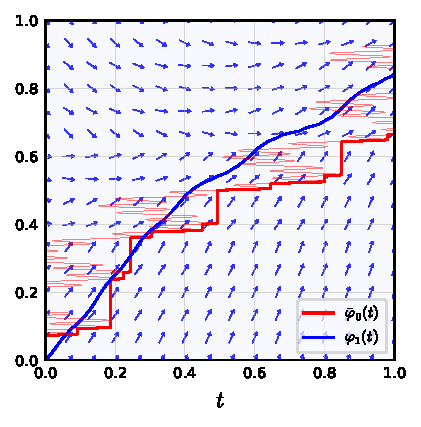
\includegraphics[width=0.48\linewidth]{figures/limit_n1}
    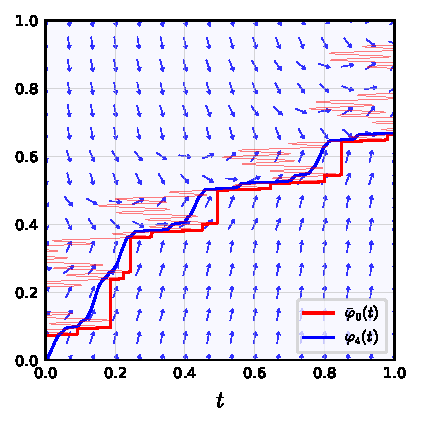
\includegraphics[width=0.48\linewidth]{figures/limit_n4}

    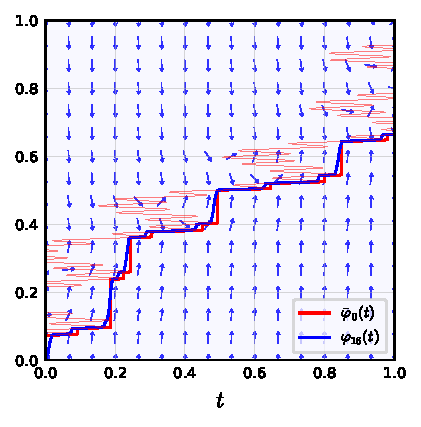
\includegraphics[width=0.48\linewidth]{figures/limit_n16}
    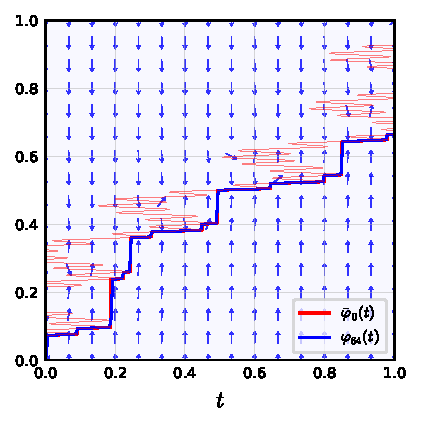
\includegraphics[width=0.48\linewidth]{figures/limit_n64}
    \caption{The convergence $\vp_n\xrightarrow{n\to\infty}\bvp_0$ on $(\bPhi,d_{\bPhi})$ of integrated CIR paths $\vp_n$ to an IG L\'evy path $\bvp_0$, as in \autoref{ex:CIR_to_IG}, is illustrated for $n=1,4,16$ and 64.}
    \label{fig:exit_converge}
\end{figure}

\begin{example}[Pathwise integrated CIR to IG]\label{ex:CIR_to_IG}
    Assume $\sigma,\kappa,\theta,v>0$ and $w\in\uC_0(\RR_+,\RR)$, and define $\{g_n\}_{n\in\NN}\subset\uC(\RR_+^2,\RR)$ by $g_n(t,x) := \sigma w(x) + \kappa\left(\theta t - x\right) + v/n$ respectively. Note $g_1$ coincides with the Heston function in \autoref{eq:hest_ode}. Then $\Vert g_0-g_n\Vert_{\RR_+^2}\xrightarrow{n\to\infty}0$, where
    \begin{equation}
        g_0(t,x) := \sigma w(x) + \kappa\left(\theta t - x\right).
    \end{equation}
    Using \autoref{def:mod_driving_func}, it is straightforward to confirm $\{g_n\}_{n\in\NN_0}\subset\uG$ provided $w$ verifies the condition $\sup_{x\in\RR_+}\kappa x - \sigma w(x)=\infty$. Equivalently, provided the function $\bvp_0$ specified by
    \begin{equation}\label{eq:exit_limit}
        \bvp_0(t) := \inf\{x>0:g_0(t,x)<0\} = \inf\{x>0: \kappa x - \sigma w(x) > \kappa\theta t\}
    \end{equation}
    is a well-defined path in $\uD(\RR_+,\RR)$. Note these conditions are met a.s.~when $w=W^1(\omega)$ is a sample path of Brownian motion. The conditions to apply \autoref{thm:exit_limit} are thus met. This tells us that $\vp_n\xrightarrow{n\to\infty} \bvp_0$ on the exit-time space $(\bPhi,d_{\bPhi})$, where each $\vp_n$ solves the IVP $x'=ng_n(t,x)$, $x(0)=0$. That is, $\vp_n$ is the unique path in $\Phi$ which verifies $\vp_n(0)=0$ and
    \begin{equation}\label{eq:ode_verify}
        \vp'_n(t) = n\sigma w(\vp_n(t)) - n\kappa(\theta t - \vp_n(t)) + v.
    \end{equation}
\end{example}

Since each $\vp_n$ can be considered a sample path of an integrated CIR process $\int_0^\cdot V_s(\omega)\dd s$ as in \autoref{eq:tce}, and the limit $\bvp_0$ a sample path of the IG Le\'vy process as in \autoref{eq:ig_intro}, we have thus established the pathwise convergence of such processes on $(\bPhi,d_{\bPhi})$, and provided a pathwise origin for \autoref{thm:mech_pro} applicable to the related Heston and NIG processes.

\begin{figure}[H]
    \centering
    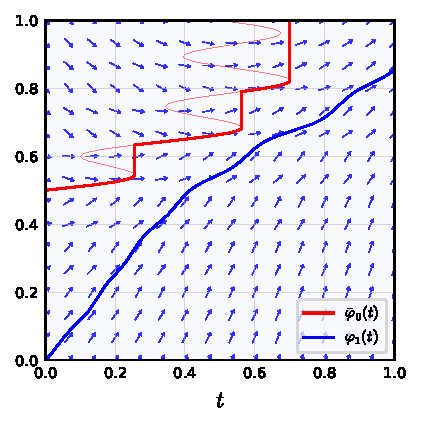
\includegraphics[width=0.48\linewidth]{figures/limit2_n1}
    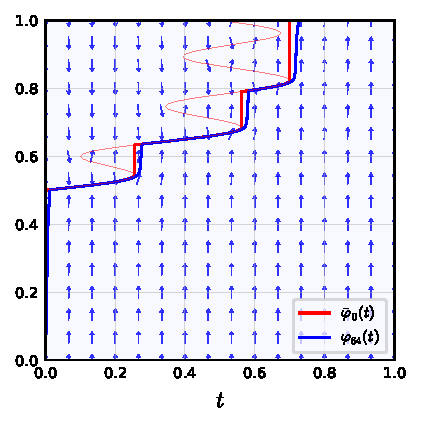
\includegraphics[width=0.48\linewidth]{figures/limit2_n64}
    \caption{The convergence in \autoref{fig:exit_converge} is repeated using $g_n(t,x) := \sigma w(x) + \kappa\left(\theta t - x\right) + v$ in \autoref{ex:CIR_to_IG} instead and truncating $w$ sooner, like in \autoref{fig:main_examples2}.}
    \label{fig:exit_converge2}
\end{figure}

This convergence is illustrated in \autoref{fig:exit_converge}, with $w$ a truncated Weierstrass path from \autoref{eq:truncated_weierstrass}. For the graphs labelled $\bvp_0(t)$ we actually use those of the interval-valued paths $\bvp_*(t):=[\bvp_0(t_-),\bvp_0(t)]$ like in \autoref{fig:function_zeros}, which coincide with the graphs of $E(\bvp_0)(x)=M(\phi_0)(x)$ by \autoref{cor:exit_lower} and help visualise $d_{\bPhi}(\vp_n,\bvp_0) \xrightarrow{n\to\infty} 0$, i.e.~uniform convergence in \emph{time} over compacts in \emph{space}. In \autoref{fig:exit_converge2} we assume $g_n(t,x) := \sigma w(x) + \kappa\left(\theta t - x\right) + v = g_0(t,x)$ instead. Contrasting \autoref{eq:exit_limit} and \cite{mechkov_2015}, a discontinuity at $t=0$ is then ensured for any chosen $w\in\uC_0(\RR_+,\RR)$ provided $v>0$, and this discontinuity has size
\begin{equation}
    \bvp_0(0) = \inf\{x>0: \kappa x - \sigma w(x) > v\}.
\end{equation}

\subsection{Excursionary limits}\label{sec:excursionary_limits}

The previous section was concerned with limits of sequences of solutions $\vp$ of the IVPs in \autoref{prob:ivp2}. As outlined in \autoref{ch:intro}, in \autoref{chap:framework} we define a framework in which price processes admit the representation $S=\exp(W^\rho_X-\frac12 X)$, where the cumulative variance process $X=\{X_t\}_{t\in\RR_+}$ here solves \autoref{prob:ivp2} on a pathwise basis. Notice that $S$ just derives from $X$ through a simple (albeit random) composition with geometric Brownian motion $\Lambda_x:=\exp(W^\rho_x-\frac12 x)$, i.e.~$S=\Lambda\circ X$. So to understand how paths of $S$ behave under the exit-time limits of \autoref{sec:bounds_limits}, we focus here primarily on the behaviour of compositions $w\circ\vp$ for some $w\in\uC(\RR_+,\RR)$, possibly related to $\vp$, under the limits of \autoref{sec:bounds_limits}. Such compositions $w\circ\vp$ do not \emph{have} to represent price paths, but could be a functional of such, like a derivative payoff. We find that instantaneous \emph{excursions} can develop in such composite limits, and these conclusions will allow us the extend the pathwise CIR and IG relationship in \autoref{ex:CIR_to_IG} to answer the Heston and NIG related questions raised in the \hyperlink{prologue}{Prologue}.

Towards understanding these composite limits, the following is reassuring and should be kept in mind. This just uses the fact that the discontinuities of a limit $\bvp_0$ on $(\bPhi,d_{\bPhi})$ are at most countable, as discussed prior to \autoref{cor:ae_converge}. Thus $\bvp_0$ is a.e.~continuous, and this can be extended to this corollary essentially by definition of $w$ being assumed continuous.
\begin{corollary}[A.e.~composite convergence]\label{cor:ae_composite}
    Suppose $\vp_n\xrightarrow{n\to\infty}\bvp_0$ on $(\bPhi,d_{\bPhi})$ and also $w\in\uC(\RR_+,\RR)$. Then for any $T\in\RR_+$ the following pointwise convergence a.e.~takes place
    \begin{equation}
        \Leb\left[t\in[0,T]: (w\circ\vp_n)(t)\xrightarrow{n\to\infty}(w\circ\bvp_0)(t)\right] =T.
    \end{equation}
\end{corollary}
This clearly leads also to integral convergences like the $\uL_p$ statements of \autoref{cor:ae_converge}. Although reassuring, the limitations of this result must be understood, because it turns out related convergences of path-dependent functionals can be violated, for example we find
\begin{equation}\label{eq:barrier_violation}
    \lim_{n\to\infty}\sup_{t\in[0,T)}(w\circ\vp_n)(t) \ge \sup_{t\in[0,T)}(w\circ\bvp_0)(t)
\end{equation}
with a strict inequality in cases of practical interest. This is an important example in practice, as it relates to the payoff of a common barrier option, albeit continuously-monitored. The analysis of this section will allow us to understand such limits, and in this example we obtain the following surprising yet fairly elegant convergence on $(\RR,|\cdot|)$ for any $T>0$
\begin{equation}\label{eq:def_barrier}
    \sup_{t\in[0,T)}(w\circ\vp_n)(t) \xrightarrow{n\to\infty} \sup_{t\in[0,T)}\sup\ (w\bullet\bvp_0)(t),\quad (w\bullet\bvp_0)(t) := \{w(x):x\in[\bvp_0(t_-),\bvp_0(t)]\}.
\end{equation}
The path $w\bullet\bvp_0$ is set-valued, hence $\sup\sup$ above, in fact compact \emph{interval}-valued. Indeed we have the following equivalent representation, noting $\bvp_*$ was utilised earlier in \autoref{fig:function_zeros},
\begin{equation}
    (w\bullet\bvp_0)(t) = \left[\min_{x\in\bvp_*(t)}w(x),\max_{x\in\bvp_*(t)}w(x)\right],\quad \bvp_*(t):=[\bvp_0(t_-),\bvp_0(t)].
\end{equation}
Such paths $w\bullet\bvp_0$ were discussed briefly in \autoref{ch:intro}, and now the emergence of an interval-valued process from the Heston model, as discussed in the \hyperlink{prologue}{Prologue}, should seem plausible.

So in general the convergence of compositions $w\circ\vp_n\xrightarrow{n\to\infty}w\circ\bvp_0$ is violated on all reasonable metric spaces on $\uD(\RR_+,\RR)$, like those of \cite{skorokhod_1956}, despite having $\vp_n\xrightarrow{n\to\infty}\bvp_0$ on $(\bPhi,d_{\bPhi})$ as in \autoref{sec:bounds_limits}. Hence the introduction of interval-valued paths, which we name \emph{excursionary}. This naming is inspired by Chapter 15 of \cite{whitt_2002}, the aim of which is to understand processes with similar paths with excursions, arising in queuing applications.

\vspace{3mm}\textbf{The excursionary space.} We now properly define our set $\uE$ of excursionary paths, then the relevant metric $d_\uE$ on it, which should be thought of as characterising the convergence of graphs over compacts in $\RR_+\times\RR$ w.r.t.~Hausdorff distances. On the resulting excursionary space $(\uE,d_\uE)$, we will obtain the functional convergence $w\circ\vp_n \xrightarrow{n\to\infty} w\bullet\bvp_0$ which \emph{cannot} be obtained on $\uD(\RR_+,\RR)$, generalising the specific limit given in \autoref{eq:def_barrier} on $(\RR,|\cdot|)$.

\begin{definition}[Set $\uE$ of paths]\label{def:excursionary_paths}
    Let the set $\uE$ contain real compact interval-valued paths $\ve$ over $\RR_+$, i.e.~which for each $t\in\RR_+$ returns a compact interval $\ve(t)=:[\ve_-(t),\ve_+(t)]\subset\RR$.
\end{definition}

For such a path $\ve$, having $\ve_-(t)=\ve_+(t)$ is acceptable, in which case $\ve(t)$ returns a singleton. Alternatively, supposing $\ve\in\uD:=\uD(\RR_+,\RR)$, then the path which returns a singleton $\{\ve(t)\}$ for each $t\in\RR_+$ is in $\uE$, which will still be labelled $\ve$ when convenient. In this sense, $\uD\subset\uE$.

We are especially interested in paths $\ve_\bullet\in\uE$ which for some $\ve_\circ\in\uD$ verifies $\ve_\bullet(t)=\{\ve_\circ(t)\}$ whenever $\ve_\circ(t_-)=\ve_\circ(t)$ and $[\ve_\circ(t_-)\wedge \ve_\circ(t),\ve_\circ(t_-)\vee \ve_\circ(t)]\subseteq \ve_\bullet(t) = [\ve_-(t),\ve_+(t)]$ otherwise. Recall that such inclusions were discussed following \autoref{eq:intro_limit_def}, which defines an excursionary generalisation $S^\bullet_t$ of the exponentiated NIG process arising from the Heston model. Unlike $\ve\in\uE$ in general, these excursionary paths $\ve_\bullet$ related to some $\ve_\circ\in\uD$ fall into the setting of Section 15.4 in \cite{whitt_2002}, and Theorem 15.4.1 there provides conditions for such paths to define a separable space when equipped with our Hausdorff metric $d_\uE$.

Towards defining this metric $d_\uE$, for $\ve\in\uE$ let its graph $\Gamma_T(\ve)$ over $[0,T]\subset\RR_+$ be defined
\begin{equation}\label{eq:graphs_deriv}
    \Gamma_T(\ve):= \{(t,x)\in[0,T]\times\RR:x\in \ve(t)\},
\end{equation}
and then define the extended graph $\Gamma^*_T(\ve):=\Gamma_T(\ve)\cup\{T\}\times\RR$ to alleviate issues at the arbitrary endpoint $T$, like we did to help define $d_{\uM_1}$ in \autoref{thm:m1_relationship}. This explains why the endpoint was removed manually in the example of \autoref{eq:def_barrier}. Now $d_\uE$ is defined thus.

\begin{definition}[Excursionary metric]\label{def:excursionary_metric}
    For $\ve_1,\ve_2\in\uE$ and $T\in\RR_+$, let the excursionary pseudometric $d_{\uE,T}$ return the Hausdorff distance $d_\uH$ between graphs $\Gamma_{1,2}:=\Gamma^*_T(\ve_{1,2})$, i.e.~
    \begin{multline}\label{eq:hausdorff_dist}
        d_{\uE,T}(\ve_1,\ve_2) := d_{\uH}(\Gamma_1,\Gamma_2) :=\\ \max\left\{\sup_{(t,x)\in\Gamma_1}\inf_{(s,u)\in\Gamma_2} |(t,x) - (s,u)|,\sup_{(t,x)\in\Gamma_2}\inf_{(s,u)\in\Gamma_1} |(t,x) - (s,u)|\right\}.
    \end{multline}
    Then define the excursionary metric $d_\uE$ on $\uE$ by $d_\uE(\ve_1,\ve_2):=\sum_{n\in \NN}2^{-n}(1\wedge d_{\uE,n}(\ve_1,\ve_2))$.
\end{definition}

Note that, like each $d_{\uE,T}$, $d_\uE$ actually defines another pseudometric on $\uE$, which is often the case with Hausdorff distances. To see this, simply consider $\ve_{1,2}\in\uE$ with $\ve_1(t):=[-1,1]$ over $\RR_+$ but $\ve_2(t):=[-1,1]$ only at the rationals $\QQ_+$, with $\ve_2(t):=\{0\}$ otherwise. Then clearly $d_\uE(\ve_1,\ve_2)=0$ but $\ve_1\neq \ve_2$. The pseudometric space $(\uE,d_\uE)$ can be upgraded to a bona fide metric space by the usual consideration of \emph{equivalence classes} of paths in $\uE$. Doing so explicitly is not actually necessary, however, given that $d_\uE$ certainly induces a Borel $\sigma$-algebra $\cE$ as usual on $\uE$, making the (pseudometrisable) topological space $(\uE,\cE)$ also a measurable space, thus suitable for our probabilistic volatility-related applications.

\vspace{2mm} Before characterising excursionary limits of composite paths $w\circ\vp$, where $\vp\in\Phi$ solves \autoref{prob:ivp2}, we first study limits of time derivatives $\vp'$. Such limits are not only helpful in their own right, given they capture the behaviour of volatility paths $\sqrt{\vp'}$, but can often be \emph{related} to composite limits. This can be seen in the Heston example in \autoref{eq:ode_verify}, or more generally when $g(t,x):=\vt(t)-w(x)$ as in \autoref{thm:solutionmap}, because then we simply find
\begin{equation}\label{eq:deriv_composite}
    (w\circ\vp)(t) = \vt(t) - \vp'(t).
\end{equation}
As already noted, in this section we will for convenience use $\vp'$ and $w\circ\vp$ to also denote the \emph{singleton}-valued paths in $\uE$, the latter coinciding with $w\bullet\vp$ defined in \autoref{eq:def_barrier}. The theory developed here will always be applied in the setting of \autoref{thm:exit_limit}, so although not strictly required the reader may adopt the assumptions there throughout: $\{g_n\}_{n\in\NN_0}\subset\uG$ is such that $\Vert g_0 - g_n \Vert_{\RR_+^2}\xrightarrow{n\to\infty}0$, $\{\vp_n\}_{n\in\NN}\subset\Phi$ respectively solve $x'=ng_n(t,x)$, $x(0)=0$ from \autoref{prob:ivp2}, and most importantly $d_{\bPhi}(\vp_n,\bvp_0)\xrightarrow{n\to\infty}0$, where $\bvp_0\in\bPhi$ is as in \autoref{thm:wellposed}.

\vspace{3mm}\textbf{Derivatives' limits.} \autoref{cor:construct_limit} constructs \emph{any} path $\bvp_0\in\bPhi\subset\uD(\RR_+,\RR)$ as a limit of solutions $\vp_n$ to \autoref{prob:ivp2}, on $(\bPhi,d_{\bPhi})$. Supposing $\bvp_0$ has a discontinuity in $(0,T)$, then we must find $\Vert \vp'_n \Vert_{[0,T]}\xrightarrow{n\to\infty}\infty$, and it is clear we should not attempt to find a limit of $\vp'_n$ as $n\to\infty$ on $\uC$, $\uD$ or even $\uE$, so neither for volatility $\sqrt{\vp'_n}$. The best we achieve here are limits of the scaled paths $n^{-1}\vp'_n$ on $(\uE,d_{\uE})$, and the approach towards this via explicit parametric representations is applied also to compositions $w\circ\vp_n$, often related like in \autoref{eq:deriv_composite}.

For the next result, keep in mind that if $\vp\in\Phi$ is a global solution of \autoref{prob:ivp2}, then the derivative $\vp'$ admits the trivial parametric representation $(\id,\vp')$, and this is in the same equivalence class as $(\vp^{-1},\vp'\circ\vp^{-1})$. This just amounts to the following equivalence in $\RR_+^2$
\begin{equation}\label{eq:deriv_equiv}
    \{(t,\vp'(t)):t\in\RR_+\} = \{(\vp^{-1}(x),\vp'(\vp^{-1}(x))):x\in\RR_+\}.
\end{equation}
Given that limits for temporal components like $\vp^{-1}$ are understood through \autoref{thm:exit_limit}, the focus in \autoref{thm:para_deriv} is the spatial component $\vp'\circ\vp^{-1}$. For clarity, in \autoref{eq:para_limit} define the path $g_0(E(\bvp_0),\id):x\mapsto g_0(E(\bvp_0)(x),x)$ in $\uC(\RR_+,\RR)$, and let the norm $\Vert\cdot\Vert_{\RR_+}$ be defined as usual using \autoref{def:uni_metric}, which characterises uniform convergence over compacts.

\begin{lemma}[Parametric derivative limits]\label{thm:para_deriv}
    Adopt the assumptions of \autoref{thm:exit_limit}, so $\vp_n\xrightarrow{n\to\infty}\bvp_0$ on $(\bPhi,d_{\bPhi})$. Then the following convergence of derivatives $\{\vp'_n\}_{n\in\NN}$ takes place~
    \begin{equation}\label{eq:para_limit}
        \left\Vert g_0(E(\bvp_0),\id) - n^{-1}\vp'_n\circ\vp_n^{-1}\right\Vert_{\RR_+} \xrightarrow{n\to\infty}  0.
    \end{equation}
\end{lemma}
\begin{proof}
    Given $\vp_n$ is the unique global solution of the IVP $x'=ng_n(t,x)$, $x(0)=0$, then $\vp'_n(t)=ng_n(t,\vp_n(t))$ is verified for each $t\in\RR_+$. Substituting $t=\vp^{-1}_n(x)$ into this, we see
    \begin{equation}
        n^{-1}\vp_n'(\vp_n^{-1}(x)) = g_n(\vp^{-1}_n(x),x)
    \end{equation}
    for each $x\in\RR_+$. The proof will thus be complete, just by definitions, if the convergence
    \begin{equation}\label{eq:converge_composite}
        \delta_n := \left\Vert g_0(E(\bvp_0),\id) - g_n(\vp^{-1}_n,\id)\right\Vert_{[0,X]} \xrightarrow{n\to\infty}  0
    \end{equation}
    takes place for all $X\in\RR_+$. We already have both $\Vert E(\bvp_0)-\vp^{-1}_n \Vert_{[0,X]}\xrightarrow{n\to\infty} 0$ and $\Vert g_0 - g_n \Vert_{[0,T]\times[0,X]}\xrightarrow{n\to\infty} 0$ for all $T,X\in\RR_+$ from \autoref{thm:exit_limit}, and these indeed combine to give \autoref{eq:converge_composite}. A modulus of continuity for $g_0\in\uC(\RR^2,\RR)$ will be utilised to show this.

    Toward this, fix $X\in\RR_+$ and $T>E(\bvp_0)(X)$. Then $\Vert E(\bvp_0)-\vp^{-1}_n \Vert_{[0,X]}<T-E(\bvp_0)(X)$ for all sufficiently large $n$, so assume w.l.o.g. $\Vert\vp_n^{-1}\Vert_{[0,X]} = \vp_n^{-1}(X)<T$ for all $n$. This means the paths of all $(\vp_n^{-1},\id)$ over $[0,X]$, which appear as arguments in \autoref{eq:converge_composite}, are bounded into the rectangle $\cX:=[0,T]\times[0,X]$. Notice that the triangle inequality gives
    \begin{equation}\label{eq:triangle_deriv}
        \delta_n \le \Vert g_0(E(\bvp_0),\id) - g_n(E(\bvp_0),\id)\Vert_{[0,X]} + \Vert g_n(E(\bvp_0),\id) - g_n(\vp^{-1}_n,\id)\Vert_{[0,X]}.
    \end{equation}
    Treating the first component here is simple, as it is clearly bounded by $\Vert g_0 - g_n\Vert_\cX$. For the second, let $w_0:\RR_+\to\RR_+$ be a modulus of continuity of $g_0$ over $\cX$, so we have the bound
    \begin{equation}\label{eq:mod_cont2}
        |g_0(t,x) - g_0(s,u)| \le w_0(|(t,x) - (s,u)|)
    \end{equation}
    for all $(t,x),(s,u)\in\cX$, and $w_0(\ep)\xrightarrow{\ep\downarrow0}0$. Using the triangle inequality twice, the relationship of \autoref{eq:mod_cont2} can be extended to each $g_n$ and $w_n$, provided we define $w_n:=w_0 + 2\Vert g_0-g_n\Vert_\cX$. Note that $w_n$ is \emph{not} a modulus of continuity for $g_n$ over $\cX$, because $w_n(\ep)\xrightarrow{\ep\to 0}2\Vert g_0-g_n\Vert_\cX\neq0$. Nevertheless, we can now bound the last term in \autoref{eq:triangle_deriv}, using
    \begin{equation}
        \Vert g_n(E(\bvp_0),\id) - g_n(\vp^{-1}_n,\id)\Vert_{[0,X]} \le w_0(\Vert E(\bvp_0)-\vp^{-1}_n \Vert_{[0,X]}) + 2\Vert g_0 - g_n\Vert_\cX.
    \end{equation}
    So in full, the claimed convergence in \autoref{eq:converge_composite} takes place because for every $X\in\RR_+$
    \begin{equation}
        \left\Vert g_0(E(\bvp_0),\id) - n^{-1}\vp'_n\circ\vp_n^{-1}\right\Vert_{[0,X]} = \delta_n \le w_0(\Vert E(\bvp_0)-\vp^{-1}_n \Vert_{[0,X]}) + 3\Vert g_0 - g_n\Vert_\cX \xrightarrow{n\to\infty}  0.
    \end{equation}
    Given $X$ is arbitrary, this extends to the claim in \autoref{eq:para_limit} w.r.t.~the norm $\Vert\cdot\Vert_{\RR+}$.
\end{proof}

Letting $\{\ve_n\}_{n\in\NN}\subset\uE$ be defined by the singletons $\ve_n(t):=\{n^{-1}\vp'(t)\}$, thus capturing the behaviour of volatility $\sqrt{\vp'}$, in \autoref{cor:hausdorff_deriv} we now combine \autoref{thm:exit_limit} and \autoref{thm:para_deriv} to obtain a surprising limit $\ve_n\xrightarrow{n\to\infty}\ve_0$ on the excursionary space $(\uE,d_\uE)$. Our approach to this, which will be repeated for the composite paths $w\circ\vp_n$ in \autoref{cor:graph_hausdorff}, is to define helpful parametric representations $(\tau_n,\sigma_n)$ of each $\ve_n$, and to establish the product uniform convergence (over compacts) of these to a limit $(\tau_0,\sigma_0)$, finally interpreting this limit as a path $\ve_0$ in $\uE$. It is intuitive that this uniform convergence of parametric representations indeed provides convergence on $\uE$ w.r.t.~Hausdorff distances, and this can be confirmed easily enough by noting that, within the definition of $d_\uE$ in \autoref{eq:hausdorff_dist} we have the bound
\begin{multline}
    \sup_{(t,x)\in\Gamma_n}\inf_{(s,u)\in\Gamma_0} |(t,x) - (s,u)| = \sup_{s\in[0,1)}\inf_{u\in[0,1)} |(\tau_n(s),\sigma_n(s)) - (\tau_0(u),\sigma_0(u))|\\
    \le \sup_{s\in[0,1)} |(\tau_n(s),\sigma_n(s)) - (\tau_0(s),\sigma_0(s))| =: \Vert(\tau_0,\sigma_0) - (\tau_n,\sigma_n)\Vert_{[0,1)}
\end{multline}
where we have assumed w.l.o.g.~that the domain of all parametric representations $(\tau_n,\sigma_n)$ have been conveniently transformed into $[0,1)$. This specifically demonstrates the bound $d_{\uE,T}(\ve_n,\ve_0)\le \Vert(\tau_0,\sigma_0) - (\tau_n,\sigma_n)\Vert_{[0,1)}$, which may be extended to what we will use, namely~
\begin{equation}\label{eq:para_limit_to_excursion}
    \Vert(\tau_0,\sigma_0) - (\tau_n,\sigma_n)\Vert_{\RR_+}\xrightarrow{n\to\infty}0 \implies d_\uE(\ve_n,\ve_0)\xrightarrow{n\to\infty}0.
\end{equation}

\begin{theorem}[Excursionary derivative limits]\label{cor:hausdorff_deriv}
    Adopt the assumptions of \autoref{thm:exit_limit}, so $d_{\bPhi}(\vp_n,\bvp_0)\xrightarrow{n\to\infty}0$, and define $\{\ve_n\}_{n\in\NN}\subset\uE$ by $\ve_n(t):=\{n^{-1}\vp'_n(t)\}$ respectively. Then $d_\uE(\ve_n,\ve_0)\xrightarrow{n\to\infty}0$, where $\ve_0\in\uE$ returns the singleton $\{0\}$ a.e.~and is precisely defined by
    \begin{equation}\label{eq:def_deriv_excursion}
        \ve_0(t) := \left[0, \ve_0^+(t)\right],\quad \ve_0^+(t):=\max_{x\in\bvp_*(t)} g_0(t,x),\quad \bvp_*(t):=[\bvp_0(t_-),\bvp_0(t)].
    \end{equation}
\end{theorem}
\begin{proof}
    Combining \autoref{thm:exit_limit} and \autoref{thm:para_deriv}, we obtain the product convergence
    \begin{equation}\label{eq:uni_prod_limit}
        \Vert(E(\bvp_0),g_0(E(\bvp_0),\id)) - (\vp_n^{-1},n^{-1}\vp'_n\circ\vp_n^{-1})\Vert_{\RR_+}\xrightarrow{n\to\infty}0.
    \end{equation}
    Now set $(\tau_n,\sigma_n):=(\vp_n^{-1},n^{-1}\vp'_n\circ\vp_n^{-1})$, which, given the equivalence of graphs in \autoref{eq:deriv_equiv}, define parametric representations of each $\ve_n$ respectively. So we will obtain the claimed convergence $d_\uE(\ve_n,\ve_0)\xrightarrow{n\to\infty}0$ using \autoref{eq:para_limit_to_excursion} and \autoref{eq:uni_prod_limit} \emph{if} the path $\ve_0$ defined in \autoref{eq:def_deriv_excursion} is similarly parameterised by $(\tau_0,\sigma_0):=(E(\bvp_0),g_0(E(\bvp_0),\id))$.

    Now $E(\bvp_0)$ is in $\uN$ from \autoref{def:setN}, i.e.~defines a non-decreasing and spatially unbounded path in $\uC_0(\RR_+,\RR)$. So the graph $\Gamma_0$ of this parametric representation $(\tau_0,\sigma_0)$ has the form
    \begin{equation}\label{eq:graph_rep}
        \Gamma_0 = \left\{(t,g_0(t,x))\in\RR_+\times\RR: x\in\bvp_*(t)\right\}.
    \end{equation}
    Using the continuity of $g_0$ and the compactness of $\bvp_*(t):=[\bvp_0(t_-),\bvp_0(t)]$, we then obtain
    \begin{equation}
        \Gamma_0 = \left\{(t,x)\in\RR_+\times\RR: x\in\left[\min_{u\in\bvp_*(t)} g_0(t,u),\max_{u\in\bvp_*(t)} g_0(t,u)\right]\right\}.
    \end{equation}
    Now if we can show that $\ve^-_0(t):=\min_{x\in\bvp_*(t)} g_0(t,x)=0$ for every $t$, then we finally obtain
    \begin{equation}
        \Gamma_0 = \left\{(t,x)\in\RR_+\times\RR: x\in\left[0,\ve_+(t)\right]\right\}.
    \end{equation}
    This will provide $\Gamma_0=\{(t,x):x\in\ve_0(t)\}$, clarifying that indeed $(\tau_0,\sigma_0)$ parameterises $\ve_0$, and therefore $d_\uE(\ve_n,\ve_0)\xrightarrow{n\to\infty}0$. To confirm $\ve^-_0(t)=0$, consider \autoref{fig:exit_converge2}. At discontinuities of $\bvp_0(t)$, we see that $g(t,x)\ge0$ is ensured for all $x\in\bvp_*(t)$. Given that $g(t,\bvp_0(t_-))=g(t,\bvp_0(t)) = 0$ also follows from the continuity of $g$, then indeed $\ve^-_0(t)=0$.

    It just remains to confirm that $\ve_0(t)=\{0\}$ a.e., and this follows from $\bvp_0(t_-)=\bvp_0(t)$ a.e., given discontinuities are countable, and therefore $\ve^+_0(t)=0$ a.e., completing the proof.
\end{proof}

\vspace{2mm}We now demonstrate \autoref{cor:hausdorff_deriv} using again \autoref{ex:CIR_to_IG}. Notice that whenever a limit of $n^{-1}\vp'_n(t)$ is characterised in the setting of \autoref{thm:exit_limit}, we are equivalently characterising that of $g_n(t,\vp_n(t))=n^{-1}\vp'_n(t)$. Given \autoref{eq:ode_verify}, in \autoref{ex:CIR_to_IG} this takes the form
\begin{equation}
    \sigma (w\circ\vp_n)(t) - \kappa(\theta t - \vp_n(t)) + v/n = n^{-1}\vp'_n(t),
\end{equation}
and these paths coincide with those of a scaled CIR process $n^{-1}V(\omega):=n^{-1}\vp_n$, recalling we identified $\int_0^\cdot V_s(\omega)\dd s := \vp_n$ in \autoref{ex:CIR_to_IG}. The limit $\ve_0\in\uE$ in \autoref{cor:hausdorff_deriv} reads
\begin{equation}\label{eq:ex_limit_def}
    \ve_0(t) := \left[0, \max_{x\in\bvp_*(t)} \sigma w(x) + \kappa\left(\theta t - x\right)\right],\quad \bvp_0(t):=\inf\{x>0: \kappa x - \sigma w(x) > \kappa\theta t\},
\end{equation}
so we can interpret the instantaneous excursions of $\ve_0$ in \emph{space} as manifesting from certain excursions of the path $w$ in \emph{time} over intervals in space. The convergence of $\ve_n(t):=\{n^{-1}\vp'_n(t)\}$ to $\ve_0$ on $(\uE,d_\uE)$, as implied by \autoref{cor:hausdorff_deriv}, is demonstrated in \autoref{fig:hausdorff_deriv}. Comparing this with \autoref{fig:exit_converge}, notice excursions in $\ve_n$ indeed develop only at jumps of $\bvp_0$.

\begin{figure}[H]
    \centering
    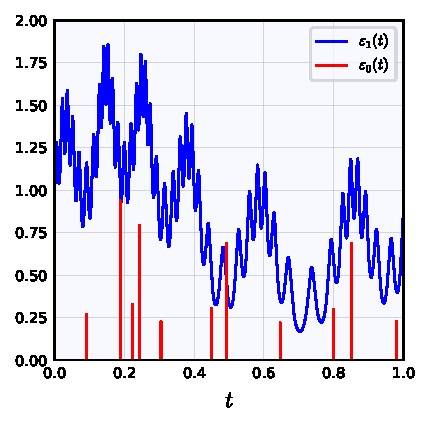
\includegraphics[width=0.48\linewidth]{figures/deriv_limit_n1}
    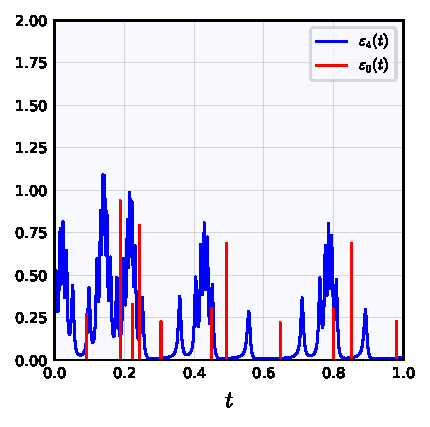
\includegraphics[width=0.48\linewidth]{figures/deriv_limit_n4}
    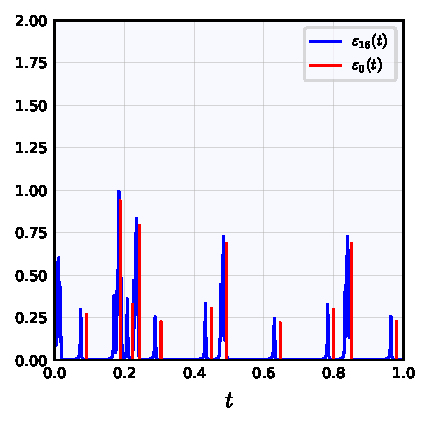
\includegraphics[width=0.48\linewidth]{figures/deriv_limit_n16}
    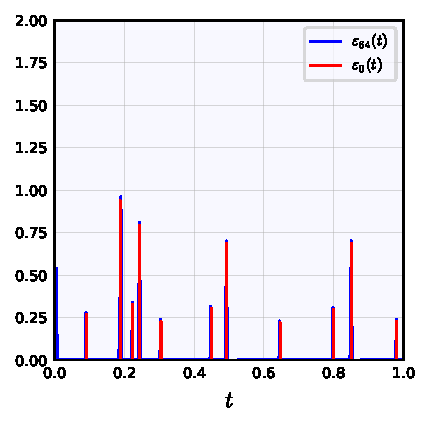
\includegraphics[width=0.48\linewidth]{figures/deriv_limit_n64}
    \caption{The convergence $\ve_n\xrightarrow{n\to\infty}\ve_0$ on $(\uE,d_\uE)$ is shown, where $\ve_n(t):=\{n^{-1}\vp'_n(t)\}$ are scaled CIR paths from \autoref{ex:CIR_to_IG}, and $\ve_0$ is defined in \autoref{eq:ex_limit_def}.}
    \label{fig:hausdorff_deriv}
\end{figure}

\vspace{3mm}\textbf{Composite limits.} Applicable to composite paths $w\circ\vp_n$, like those of our price processes $S_t:=\exp(W^\rho_{X_t}-\frac12 X_t)$ defined later, the structure of this part mirrors the last, clarifying our approach towards limiting results which derive from \autoref{thm:exit_limit}. Specifically, \autoref{thm:para_uniform} here provides the convergence of some helpful parametric representations (uniformly over compacts), and \autoref{cor:graph_hausdorff} reduces this to a result on the excursionary space $(\uE,d_\uE)$. Recall that in \autoref{cor:ae_composite} we have already demonstrated the pointwise convergence $(w\circ\vp_n)(t)\xrightarrow{n\to\infty}(w\circ\bvp_0)(t)$ a.e., so here we generalise this to (surprising) functional statements. Although we will work with a fixed path $w\in\uC:=\uC(\RR_+,\RR)$, this may be generalised to a sequence $\{w_n\}_{n\in\NN_0}$ verifying $\Vert w_0 - w_n\Vert_{\RR_+}\xrightarrow{n\to\infty} 0$ without difficulty.

For a global solution $\vp\in\Phi$ of \autoref{prob:ivp2} with inverse $\vp^{-1}$, notice that $(\id,w\circ\vp)$ and $(\vp^{-1},w)$ are in the same equivalence class of parametric representations, precisely meaning
\begin{equation}\label{eq:para_equiv}
    \{(t,w(\vp(t))):t\in\RR_+\} = \{(\vp^{-1}(x),w(x)):x\in\RR_+\}.
\end{equation}
This equivalence is analogous to that in \autoref{eq:deriv_equiv}, applicable instead to derivatives $\vp'$. The next result uses this to obtain a trivial extension of \autoref{thm:exit_limit} which nevertheless encodes what we need to appreciate the behaviour of composite paths $w\circ\vp_n$ as $n\to\infty$.

\begin{corollary}[Parametric composite limits]\label{thm:para_uniform}
    Adopt the assumptions of \autoref{thm:exit_limit}, so that $d_{\bPhi}(\vp_n,\bvp_0)\xrightarrow{n\to\infty}0$, and fix $w\in\uC(\RR_+,\RR)$. Then the sequence $\{(\vp^{-1}_n,w)\}_{n\in\NN}$ verifies
    \begin{equation}
         \left\Vert (E(\bvp_0),w) - (\vp^{-1}_n,w)\right\Vert_{\RR_+} \xrightarrow{n\to\infty}  0.
    \end{equation}
\end{corollary}
\begin{proof}
    Given the spatial components here clearly verify $\Vert w-w\Vert_{\RR_+}=0$, the claim follows just from the conclusion $d_{\bPhi}(\vp_n,\bvp_0)=\Vert E(\bvp_0)-\vp_n^{-1}\Vert_{\RR_+}\xrightarrow{n\to\infty}0$ within \autoref{thm:exit_limit}.
\end{proof}

Letting $\{\ve_n\}_{n\in\NN}\subset\uE$ be defined by the singletons $\ve_n(t):=\{(w\circ\vp_n)(t)\}$, in \autoref{cor:graph_hausdorff} we now establish a limit $\ve_n\xrightarrow{n\to\infty}\ve_0$ on the excursionary space $(\uE,d_\uE)$, thus describing the limiting behaviour of $w\circ\vp_n$ and therefore price paths also. As discussed in \autoref{ch:intro}, the limit found is of course the filled composition $\ve_0:=w\bullet\bvp_0$ defined by $(w\bullet\bvp)(t) := \{w(x):x\in\bvp_*(t)\}$ where as usual $\bvp_*(t):=[\bvp_0(t_-),\bvp_0(t)]$. Note $\ve_0(t)$ returns the singleton $\{(w\circ\bvp_0)(t)\}$ a.e., and to draw comparisons with \autoref{eq:def_deriv_excursion} we have the equivalent representation
\begin{equation}\label{eq:def_comp_excursion}
    \ve_0(t) := \left[\ve_0^-(t), \ve_0^+(t)\right],\quad \ve_0^-(t):=\min_{x\in\bvp_*(t)} w(x),\quad \ve_0^+(t):=\max_{x\in\bvp_*(t)} w(x).
\end{equation}

\begin{theorem}[Excursionary composite limits]\label{cor:graph_hausdorff}
    Adopt the assumptions of \autoref{thm:exit_limit}, so that $d_{\bPhi}(\vp_n,\bvp_0)\xrightarrow{n\to\infty}0$, and fix $w\in\uC(\RR_+,\RR)$. Define the set $\{\ve_n\}_{n\in\NN}\subset\uE$ respectively by the singletons $\ve_n(t):=\{(w\circ\vp_n)(t)\}$, and $\ve_0:=w\bullet\bvp_0\in\uE$. Then $d_\uE(\ve_n,\ve_0)\xrightarrow{n\to\infty}0$.
\end{theorem}
\begin{proof}
    From \autoref{thm:para_uniform}, we have the product convergence $\Vert(\tau_0,\sigma_0) - (\tau_n,\sigma_n) \Vert_{\RR_+} \xrightarrow{n\to\infty}  0$, where $(\tau_0,\sigma_0):=(E(\bvp_0),w)$ and $(\tau_n,\sigma_n):=(\vp^{-1}_n,w)$. So we can use the approach from \autoref{eq:para_limit_to_excursion} to obtain the claim of $d_\uE(\ve_n,\ve_0)\xrightarrow{n\to\infty}0$ \emph{if} every $(\tau_n,\sigma_n)$ parameterises $\ve_n$.

    When $n\neq0$, $(\tau_n,\sigma_n)$ clearly parameterises $\ve_n$, using the equivalence in \autoref{eq:para_equiv}. To see that $(\tau_0,\sigma_0)$ also parameterises $\ve_0$, we manipulate the graph $\Gamma_0$ of $(\tau_0,\sigma_0)$ to obtain
    \begin{multline}
        \Gamma_0 = \left\{(E(\bvp_0)(x),w(x)): x\in\RR_+\right\}\\
        = \left\{(t,w(x))\in\RR_+\times\RR: x\in[\bvp_0(t_-),\bvp_0(t)]\right\}\\
        = \left\{(t,x)\in\RR_+\times\RR: x\in(w\bullet\bvp_0)(t)\right\}.
    \end{multline}
    Given $\ve_0:=w\bullet\bvp_0$, then we may equivalently write $\Gamma_0=\{(t,x):x\in\ve_0(t)\}$ to see that $(\tau_0,\sigma_0)$ indeed parameterises $\ve_0$. So we obtain $d_\uE(\ve_n,\ve_0)\xrightarrow{n\to\infty}0$, completing the proof.
\end{proof}

To conclude this chapter, an example of \autoref{cor:graph_hausdorff} is provided which extends the pathwise CIR and IG limiting relationship from \autoref{ex:CIR_to_IG} to the Heston and NIG models, as discussed in the \hyperlink{prologue}{Prologue}. This provides a deep foundation for strengthening and generalising \autoref{thm:mech_pro} from \cite{mechkov_2015}, as we will do in \autoref{sec:price_limits}. The resulting convergence $\ve_n\xrightarrow{n\to\infty}\ve_0$ of price paths is shown in \autoref{fig:hausdorff_composite}, and is consistent with \autoref{fig:hausdorff_deriv}.

\begin{example}[Pathwise Heston to NIG]\label{ex:heston_to_NIG}
    Fix paths $w_{0,1}\in\uC_0:=\uC_0(\RR_+,\RR)$ and for some $\rho\in[-1,1]$ define $w_\rho:=\rho w_1 + \sqrt{1-\rho^2}w_0$. These can be interpreted as sample paths of the Brownian motion which defines the Heston model in \autoref{eq:tce2}, e.g.~$w_{\rho}:=W^{\rho}(\omega)$. Now let $\vp_n\in\Phi$ solve the IVPs $x'=ng_n(t,x)$, $x(0)=0$ in \autoref{ex:CIR_to_IG} with $w:=w_1$, so that
    \begin{equation}
        \vp'_n(t) = n\sigma (w_1\circ\vp_n)(t) - n\kappa(\theta t - \vp_n(t)) + v.
    \end{equation}
    Let each singleton-valued path $\ve_n\in\uE$ be defined from $w_\rho$ and the solution $\vp_n$ according to
    \begin{equation}
        \ve_n(t) := \left\{\exp\left((w_\rho\circ\vp_n)(t) - \frac12\vp_n(t)\right)\right\}.
    \end{equation}
    Using again \autoref{eq:tce2}, notice that $\ve_n$ and $\vp_n$ may then be considered as sample paths of the Heston price process and its cumulative variance respectively. As in \autoref{ex:CIR_to_IG}, \autoref{thm:exit_limit} can be applied to obtain $\vp_n\xrightarrow{n\to\infty}\bvp_0$ on $(\bPhi,d_{\bPhi})$, where $\bvp_0$ is an IG L\'evy path. Defining the geometric Brownian path $w(x):=\exp(w_\rho(x)-\frac12 x)$, we can apply \autoref{cor:graph_hausdorff} to additionally obtain the convergence $\ve_n\xrightarrow{n\to\infty}\ve_0$ on $(\uE,d_{\uE})$, where $\ve_0:=w\bullet\bvp_0$. In full,
    \begin{equation}\label{eq:pricelimit_def}
        \ve_0(t) := \left\{\exp\left(w_\rho(x)-\frac12 x\right): x\in[\bvp_0(t_-),\bvp_0(t)]\right\}.
    \end{equation}
\end{example}

\begin{figure}[H]
    \centering
    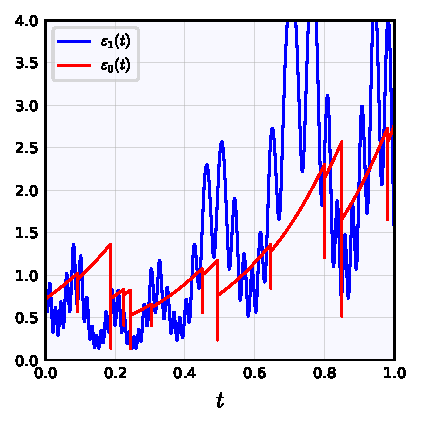
\includegraphics[width=0.48\linewidth]{figures/compose_limit_n1}
    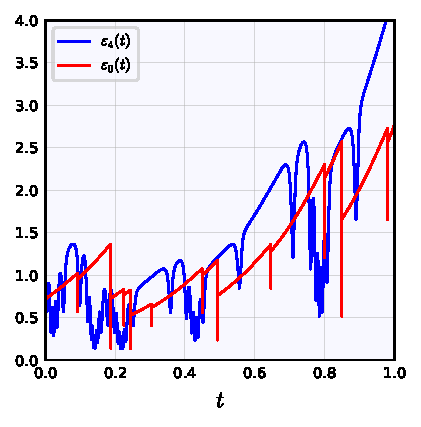
\includegraphics[width=0.48\linewidth]{figures/compose_limit_n4}
    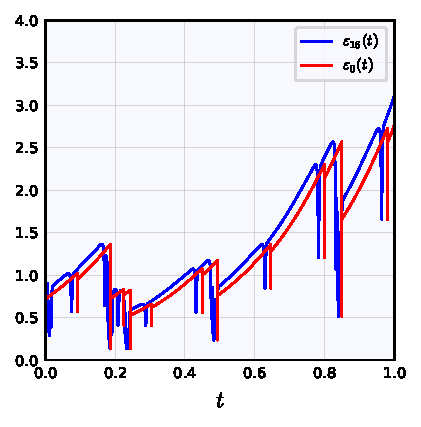
\includegraphics[width=0.48\linewidth]{figures/compose_limit_n16}
    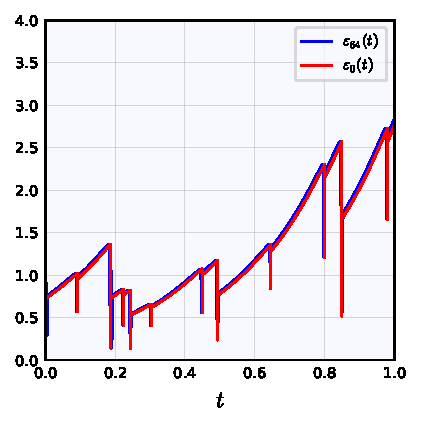
\includegraphics[width=0.48\linewidth]{figures/compose_limit_n64}
    \caption{The convergence $\ve_n\xrightarrow{n\to\infty}\ve_0$ on $(\uE,d_\uE)$ is shown, where $\ve_n$ are Heston price paths and $\ve_0$ is an interval-valued generalisation of an exponentiated NIG path, both defined in \autoref{ex:heston_to_NIG}.}
    \label{fig:hausdorff_composite}
\end{figure}

    Notice that $\ve_0$ is a path of the limit $S^\bullet$ in \autoref{eq:intro_limit_def}, which we claim is an interval-valued generalisation of the exponentiated NIG process $S^\circ$ there. This will be covered in \autoref{lem:NIG_reduc}, but notice that when $\bvp_0(t_-)=\bvp_0(t)$, which is a.e., then $\ve_0(t)$ just contains
    \begin{equation}
        \exp\left((w_\rho\circ\bvp_0)(t)-\frac12 \bvp_0(t)\right) = \exp\left(\sqrt{1-\rho^2}(w_0\circ\bvp_0)(t) + \frac{2\rho-\sigma}{2\sigma}\bvp_0(t) -\frac{\rho\theta}{\sigma} t\right)
    \end{equation}
    where the final expression uses the relationship $\kappa \bvp_0(t) - \sigma (w_1\circ\bvp_0)(t)=\kappa\theta t$ to eliminate $w_1\circ\bvp_0$, which follows from the definition of $\bvp_0$. Now clearly this expression coincides with a path of the exponentiated NIG process $S^\circ$. We have thus demonstrated the convergence of Heston price paths $\ve_n$ to paths $\ve_0$ of an interval-valued exponentiated NIG generalisation.

\vspace{4mm}For consistency, in \autoref{fig:hausdorff_composite} we fix the path $w_1$ in \autoref{ex:heston_to_NIG} to be the Weierstrass path driving \autoref{fig:hausdorff_deriv}, and set $\rho=-1$ (not unreasonable for equity prices) so there is actually no dependence on the additional path $w_0$. An interesting effect of setting $\rho=-1$ is that only \emph{downwards} excursions develop in the Heston price paths $\ve_n$, which are upwards if instead $\rho=1$. These downwards excursions are clearly evident in the generalised NIG limit $\ve_0$ in \autoref{fig:hausdorff_composite}. Through the relevant ODE, e.g.~\autoref{eq:deriv_composite}, these downwards price excursions in \autoref{fig:hausdorff_composite} can be related directly to the \emph{upwards} excursions of volatility from \autoref{fig:hausdorff_deriv}.
